\documentclass[a4paper,11pt]{article}
%included package%
\usepackage[utf8]{inputenc}
\usepackage[ngerman]{babel}
\usepackage[a4paper,left=3cm,right=3cm,top=2.5cm,bottom=2.5cm]{geometry}
%\usepackage{natbib}
\usepackage{graphicx}
\usepackage{subcaption}
\usepackage{float}
\usepackage{amsmath}
\usepackage{listings}
\usepackage{color}
\usepackage{breqn}
\usepackage{chngcntr}
\usepackage{amssymb}
\usepackage[section]{placeins}
\usepackage{hyperref}
\hypersetup{hidelinks}
\usepackage{csquotes}
\usepackage[backend=bibtex]{biblatex}
\usepackage{soul}
%for table use
\usepackage{booktabs}
\usepackage{multirow}


%bib location
\addbibresource{references.bib}


%equation counters%
\counterwithin*{equation}{section}
\counterwithin*{equation}{subsection}


%colours and stuff for the codes%
\definecolor{dkgreen}{rgb}{0,0.6,0}
\definecolor{gray}{rgb}{0.5,0.5,0.5}
\definecolor{mauve}{rgb}{0.58,0,0.82}

\lstset{frame=tb,
  language=C++,
  aboveskip=3mm,
  belowskip=3mm,
  showstringspaces=false,
  columns=flexible,
  basicstyle={\small\ttfamily},
  numbers=none,
  numberstyle=\tiny\color{gray},
  keywordstyle=\color{blue},
  commentstyle=\color{dkgreen},
  stringstyle=\color{mauve},
  breaklines=true,
  breakatwhitespace=true,
  tabsize=3
}
%end of configs%


\begin{document}
\begin{titlepage}

\newcommand{\HRule}{\rule{\linewidth}{0.5mm}} % Defines a new command for the horizontal lines, change thickness here

\center % Center everything on the page

%----------------------------------------------------------------------------------------
%	HEADING SECTIONS
%----------------------------------------------------------------------------------------

\textsc{\LARGE Technische Universität Berlin}\\[1cm] % Name of your university/college
\textsc{\Large Fraunhofer-Institut für Offene\\[0.1cm] Kommunikationssysteme FOKUS}\\[1cm] % Major heading such as course name
\textsc{\LARGE Fakultät IV}\\[1cm] % Name of your university/college
\textsc{\Large Projekt Vertiefung / Vernetztes und \\[0.1cm]Automatisiertes Fahren}\\[0.3cm]
\textsc{\Large \textbf{Sommersemester 2026}}\\[1cm]

%----------------------------------------------------------------------------------------
%	TITLE SECTION
%----------------------------------------------------------------------------------------

\HRule \\[0.4cm]
{ \huge \bfseries Multisensor LiDAR 3D Object Detection\\[0.2cm]
    \large Training and Evaluation}\\[0.4cm] % Title of your document
\HRule \\[1cm]

%----------------------------------------------------------------------------------------
%	AUTHOR SECTION
%----------------------------------------------------------------------------------------

\textsc{\large \textbf{Teammitglieder:} }\\ [0.2cm]% Minor heading such as course title

\Large Laurenz \textsc{Gilbert} (508033) \\[0.1cm]

\Large Haoran \textsc{Wang} (519707) \\[0.7cm]

\textsc{\large \textbf{Betreut von:} }\\[0.2cm] % Minor heading such as course title

\Large Johann Nikolai \textsc{Hark} \\[0.1cm]

\Large Manuel \textsc{Schiewe} \\[0.6cm]

%----------------------------------------------------------------------------------------
%	DATE SECTION
%----------------------------------------------------------------------------------------

\vfill % Fill the rest of the page with white space

{\large 31. Juli 2026} % Date, change the \today to a set date if you want to be precise

\end{titlepage}

\tableofcontents
\newpage
\section*{Sperrvermerk}
\addcontentsline{toc}{section}{Sperrvermerk}
\sloppy
Der vorgelegte Projektbericht mit dem Titel \textbf{Multisensor LiDAR 3D Object Detection: Training and Evaluation} beinhaltet vertrauliche Informationen und Daten des \textbf{Fraunhofer-Instituts für Offene Kommunikations\-systeme FOKUS sowie des DCAITI der TU Berlin}.\vspace{0.5cm}

Dieser Projektbericht darf nur vom Gutachter sowie berechtigten Mitgliedern des Prüfungsausschusses eingesehen werden. Eine Vervielfältigung und Veröffentlichung des Berichts ist auch auszugsweise nicht erlaubt.

\vspace{0.5cm}

Dritten darf diese Arbeit nur mit der ausdrücklichen Genehmigung der Verfasser und der beteiligten Institutionen zugänglich gemacht werden.

\newpage
\section*{Abkürzungsverzeichnis}
\addcontentsline{toc}{section}{Abkürzungsverzeichnis}

{\renewcommand{\arraystretch}{1.8}
\begin{tabular}{@{}ll@{}}
AP      & Average Precision \\[0.3em]
BEV     & Bird's Eye View \\[0.3em]
CV      & Cross-Validation \\[0.3em]
DCAITI  & Daimler Center for Automotive IT Innovations \\[0.3em]
fps     & frames per second \\[0.3em]
GT      & Ground Truth \\[0.3em]
ICP     & Iterative Closest Point \\[0.3em]
IoU     & Intersection over Union \\[0.3em]
LiDAR   & Light Detection and Ranging \\[0.3em]
mAP     & mean Average Precision \\[0.3em]
NMS     & Non-Maximum Suppression \\[0.3em]
OOF     & Out-of-Fold
\end{tabular}
}

\newpage
\phantomsection
\addcontentsline{toc}{section}{Abbildungsverzeichnis}
\listoffigures
\newpage
\section*{Zusammenfassung}
\addcontentsline{toc}{section}{Zusammenfassung}

In diesem Projekt wurde untersucht, wie gut vortrainierte neuronale Netze zur dreidimensionalen Objekterkennung auf eine fest installierte Zwei-Sensor-LiDAR-Anlage in einer Tiefgarage angepasst werden können. Die Zielklassen sind \textbf{Person}, \textbf{Fahrrad} und \textbf{Auto}. Verglichen wurden die beiden Einzelsensoransichten \texttt{os0} und \texttt{os1} sowie die aus beiden Sensoren erzeugte fusionierte Punktwolke \texttt{merged}.

Als Hauptmodell wurde PointPillars eingesetzt und ausgehend von einem auf KITTI vortrainierten Drei-Klassen-Checkpoint für 50 Epochen auf den Projektdaten finetuned. Wegen des starken Klassenungleichgewichts wurde eine ausschließlich aus Trainingsdaten erzeugte GT-Sampling-Datengrundlage verwendet. Die abschließende Bewertung folgt einer vor der Ergebnissichtung eingefrorenen gepaarten 3-Fold-Cross-Validation. In jedem Fold werden drei vollständige Experimente, je eines für Auto, Fahrrad und Person, als ungesehene Testaufnahmen zurückgehalten.

Die Anpassung an die Zielszene ist der entscheidende Schritt. In einem nicht kontrollierten Größenordnungsvergleich mit einer Vorgängerarbeit auf denselben Aufnahmen erreichen ausschließlich vortrainierte Modelle einen mAP von höchstens 0{,}058, das hier finetunete Modell 0{,}798. Der Abstand von 0{,}740 mAP ist je nach Ansicht sechs- bis sechzehnmal größer als der Abstand zwischen den beiden untersuchten Architekturen.

PointPillars erreicht mit der fusionierten Ansicht in jedem Fold den höchsten Gesamt-mAP. Der Fold-Mittelwert beträgt \(0{,}798 \pm 0{,}037\) für \texttt{merged}, \(0{,}777 \pm 0{,}018\) für \texttt{os0} und \(0{,}770 \pm 0{,}027\) für \texttt{os1}. Dieser Gesamtwert bewertet allerdings auch die Wiedererkennung der zahlreichen geparkten Fahrzeuge. Beschränkt auf die bewegten Objekte wächst der Vorsprung gegenüber der besseren Einzelansicht von 0{,}021 auf 0{,}040 in der offiziellen und 0{,}069 in der labelbasierten Auswertung. Der Fusionsvorteil ist moderat, aber über alle Folds konsistent und zeigt sich vor allem bei der präzisen Lokalisierung von Personen und Fahrrädern -- in beiden Auswertungsvarianten. Beim reinen Auffinden von Objekten ist die Fusion dagegen nicht überlegen: Auf den einzelnen Testexperimenten erreicht die Einzelansicht \texttt{os0} bei AP\textsubscript{30} sowohl den höchsten Mittelwert als auch die geringste Streuung. Zusätzlich wurde CenterPoint als Alternativarchitektur herangezogen; sie bestätigt die Rangfolge der Ansichten, bleibt aber in allen Ansichten hinter PointPillars zurück.

Die fusionierte Punktwolke benötigt auf der Evaluations-GPU ungefähr 85\,ms pro Modellinferenz, gegenüber 45\,ms für \texttt{os0} und 43\,ms für \texttt{os1}. Diese Messung belegt die 10-Hz-Fähigkeit der Modellinferenz, nicht jedoch die Echtzeitfähigkeit des vollständigen Fusionssystems. Die vorhandene Offline-Merge-Pipeline benötigt im Median 2{,}25\,s pro Frame; ein optimierter Online-Merge mit einmalig bestimmter Extrinsik wurde noch nicht gemessen.

\newpage
\section{Aufgabenstellung und Forschungsfragen}

Die Ausgangssituation ist eine fest installierte Verkehrsszene in einer Tiefgarage, die gleichzeitig von zwei LiDAR-Sensoren aus unterschiedlichen Perspektiven erfasst wird. Das Projekt soll ein vortrainiertes 3D-Objekterkennungsmodell auf diese Zielszene anpassen und den Nutzen der Multisensorfusion quantifizieren.

Aus der Aufgabenstellung ergeben sich vier zentrale Forschungsfragen:

\begin{enumerate}
    \item Welche Bedeutung besitzt das Finetuning auf die projektspezifischen Tiefgaragendaten gegenüber der unveränderten Übernahme eines vortrainierten Modells?
    \item Welche Unterschiede bestehen zwischen den Einzelsensoransichten \texttt{os0} und \texttt{os1} und der fusionierten Ansicht \texttt{merged}?
    \item Zeigt sich ein Fusionsvorteil eher beim bloßen Finden eines Objekts oder bei der räumlich präzisen Lokalisierung?
    \item Welche typischen Fehlerbilder und praktischen Laufzeitgrenzen besitzt die entwickelte Verarbeitungskette?
\end{enumerate}

Der Fokus liegt auf drei Klassen: Person, Fahrrad und Auto. Die wissenschaftliche Hauptaussage soll nicht aus einzelnen Beispielbildern oder einem einzigen zufälligen Split abgeleitet werden, sondern aus vollständig ungesehenen Aufnahmen unter einem für alle drei Ansichten gepaarten Protokoll.

Frage~1 wird in Abschnitt~\ref{sec:finetuning-wirkung} beantwortet, Frage~2 in den Abschnitten~\ref{sec:gesamtleistung} bis \ref{sec:generalisierung-experiment}, Frage~3 in Abschnitt~\ref{sec:bewegte-klassen} und Frage~4 in den Kapiteln~\ref{sec:fehleranalyse} und \ref{sec:laufzeit}. Abschnitt~\ref{sec:centerpoint-ergebnis} prüft ergänzend, ob die Antwort auf Frage~2 von der gewählten Modellarchitektur abhängt. Die Schlussfolgerung führt alle vier Antworten zusammen.

\newpage
\section{Datengrundlage}

\subsection{Sensoraufbau und Ansichten}

Die Szene wird von zwei Ouster-LiDAR-Sensoren mit einer Aufnahmerate von ungefähr 10\,Hz erfasst. Jeder Sensor besitzt zunächst ein eigenes Koordinatensystem. Aus den Rohdaten werden drei Eingabevarianten erzeugt:

\begin{itemize}
    \item \texttt{os0}: transformierte Punktwolke des ersten Sensors,
    \item \texttt{os1}: transformierte Punktwolke des zweiten Sensors,
    \item \texttt{merged}: geometrisch registrierte und zusammengefügte Punktwolke beider Sensoren.
\end{itemize}

Eine Einzelsensor-Punktwolke enthält typischerweise ungefähr 105.000 Punkte, die fusionierte Punktwolke ungefähr 210.000 Punkte. Abbildung~\ref{fig:setup} zeigt den Grundriss des Versuchsbereichs mit den Sensorpositionen.

\begin{figure}[H]
\centering
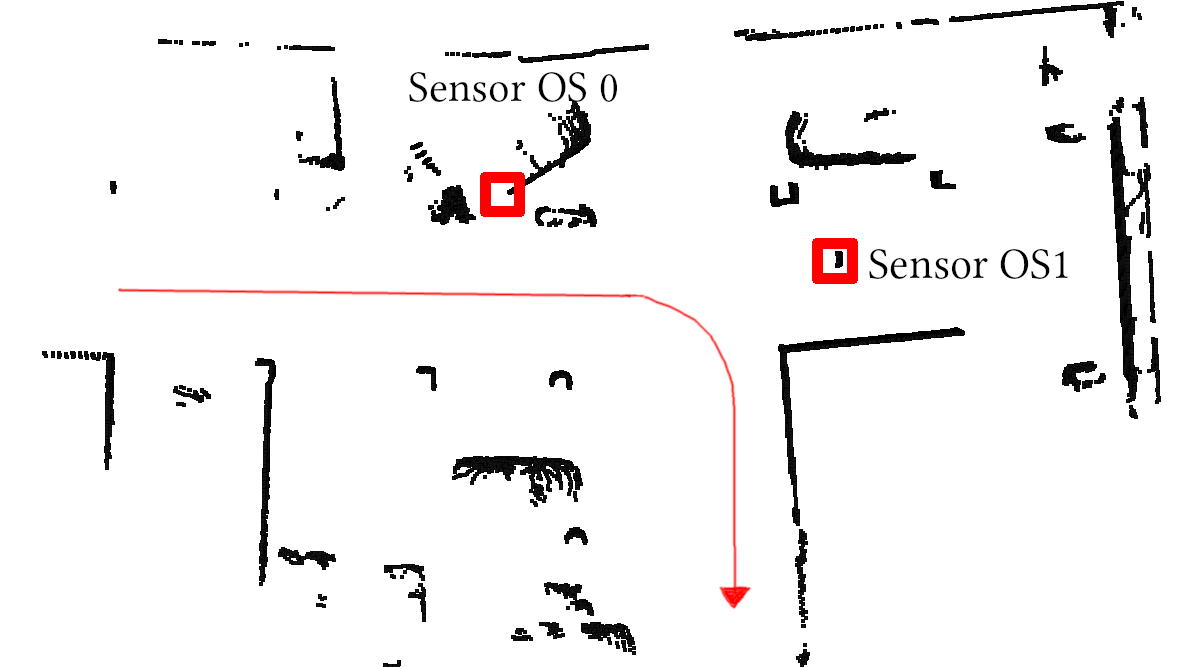
\includegraphics[width=0.85\textwidth]{images/Setup.png}
\caption{Grundriss des Versuchsbereichs in der Tiefgarage des Fraunhofer FOKUS mit den Sensorpositionen OS0 und OS1 entlang der markierten Route. Aus \cite[Abb.~21]{pagel2025railway}.}
\label{fig:setup}
\end{figure}

Die Fusion erhöht damit die Punktdichte und ergänzt verdeckte Objektseiten, vergrößert aber zugleich die zu verarbeitende Datenmenge und den sichtbaren Hintergrund.

\subsection{Aufgezeichnete Experimente}

Am 9. Oktober 2025 wurden neun Bewegungsaufnahmen in derselben Tiefgaragenszene erstellt (Tabelle~\ref{tab:experiments}):

\begin{table}[H]
\centering
\begin{tabular}{cc}
\toprule
\textbf{Experimente} & \textbf{Bewegte Zielklasse} \\
\midrule
1--3 & Auto \\
4--6 & Fahrrad \\
7--9 & Person \\
\bottomrule
\end{tabular}
\caption{Aufgezeichnete Experimente und die jeweils bewegte Zielklasse.}
\label{tab:experiments}
\end{table}

Neben dem jeweiligen bewegten Zielobjekt enthält die Szene zahlreiche statische Objekte, insbesondere geparkte Fahrzeuge. Diese statischen Objekte sind für eine realistische Detektion relevant, dürfen bei der Interpretation der Generalisierungsleistung aber nicht mit vollständig neuen Objektinstanzen verwechselt werden: Sie stehen über viele Aufnahmen hinweg an denselben Positionen.

Für die abschließende Cross-Validation wird ausschließlich die Schnittmenge der gültigen Zeitstempel aller drei Ansichten verwendet. Dadurch erhält jede Ansicht dieselben 2.122 physischen Frames. Die Annotationen bleiben dennoch ansichtsspezifisch, weil ein Objekt je nach Sensorabdeckung und Sichtbarkeit nicht in jeder Ansicht in exakt denselben Frames annotiert ist.

\subsection{Annotationen}

Die Ground-Truth-Annotationen bestehen aus orientierten dreidimensionalen Bounding Boxes. Für jede Box werden Klasse, Position, Abmessungen und Orientierung gespeichert. Zusätzlich kennzeichnet ein \texttt{static}-Attribut statische Objekte. Die finalen Labels wurden mit dem projektspezifischen Editor \texttt{experiment/manual\_bbox\_editor.py} geprüft und korrigiert (Abbildung~\ref{fig:manual-labeling}).

\begin{figure}[H]
\centering
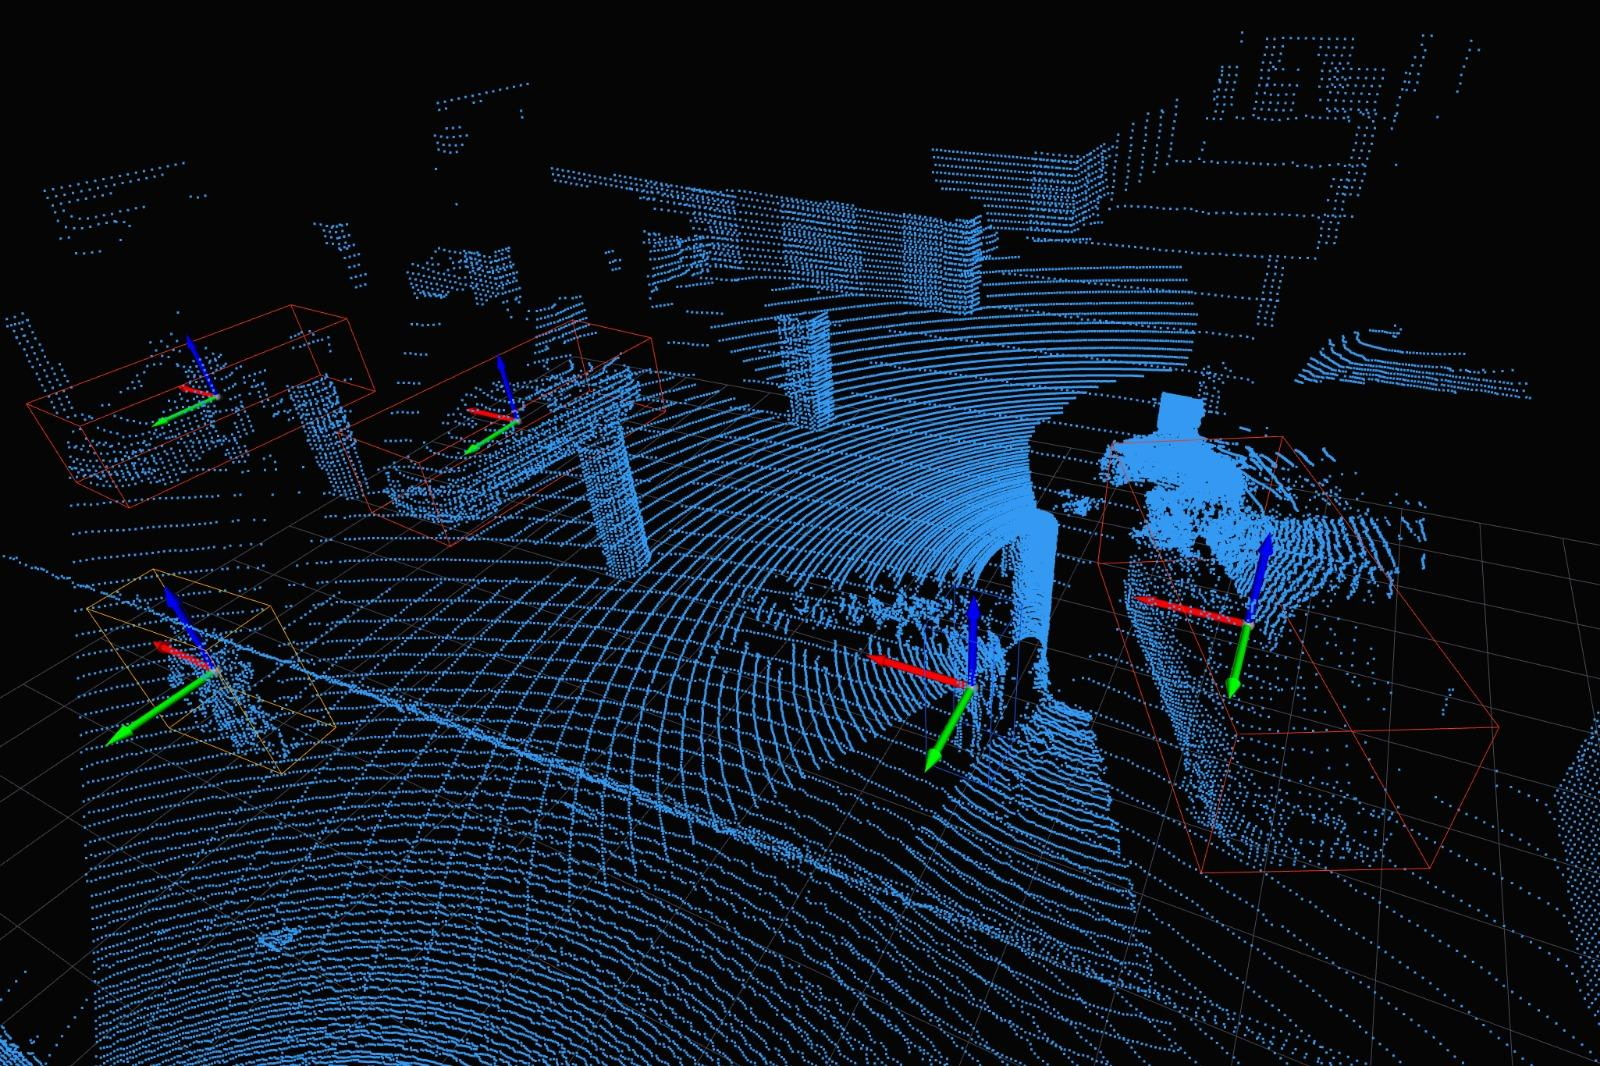
\includegraphics[width=0.95\textwidth]{images/manual-labeling.png}
\caption{Manuelle Nachbearbeitung der Ground-Truth-Annotationen mit dem projektspezifischen Bounding-Box-Editor. Dargestellt ist eine Punktwolke mit orientierten 3D-Boxen für die Klassen Person, Fahrrad und Auto.}
\label{fig:manual-labeling}
\end{figure}

Die ansichtsspezifischen Annotationen sind für den regulären Betrieb sinnvoll, begrenzen aber einen direkten Klassenvergleich zwischen den Ansichten. Beim bewegten Auto ist die Vergleichsmenge exakt gepaart (\(n=339\) in jeder Ansicht). Bei Person und Fahrrad unterscheiden sich die GT-Zahlen. Beispielsweise enthält die gepoolte Fahrradauswertung 718 Instanzen für \texttt{merged}, 627 für \texttt{os0} und 581 für \texttt{os1}.

Diese Differenz ist besonders wichtig für die Interpretation des Fahrrad-AP\textsubscript{30}: \texttt{os0} wird teilweise nur auf dem kürzeren, gut sichtbaren Abschnitt einer Trajektorie bewertet, während \texttt{merged} durch die größere Abdeckung zusätzliche und weiter entfernte Objektpositionen enthält. Der AP\textsubscript{30}-Vorsprung von \texttt{os0} darf deshalb nicht ohne Einschränkung als grundsätzliche Überlegenheit eines Einzelsensors interpretiert werden.

\newpage
\section{Datenaufbereitung und Sensorfusion}

Abbildung~\ref{fig:pipeline} gibt einen Überblick über die gesamte Verarbeitungskette. Die einzelnen Schritte werden in den folgenden Abschnitten detailliert beschrieben.

\begin{figure}[H]
\centering
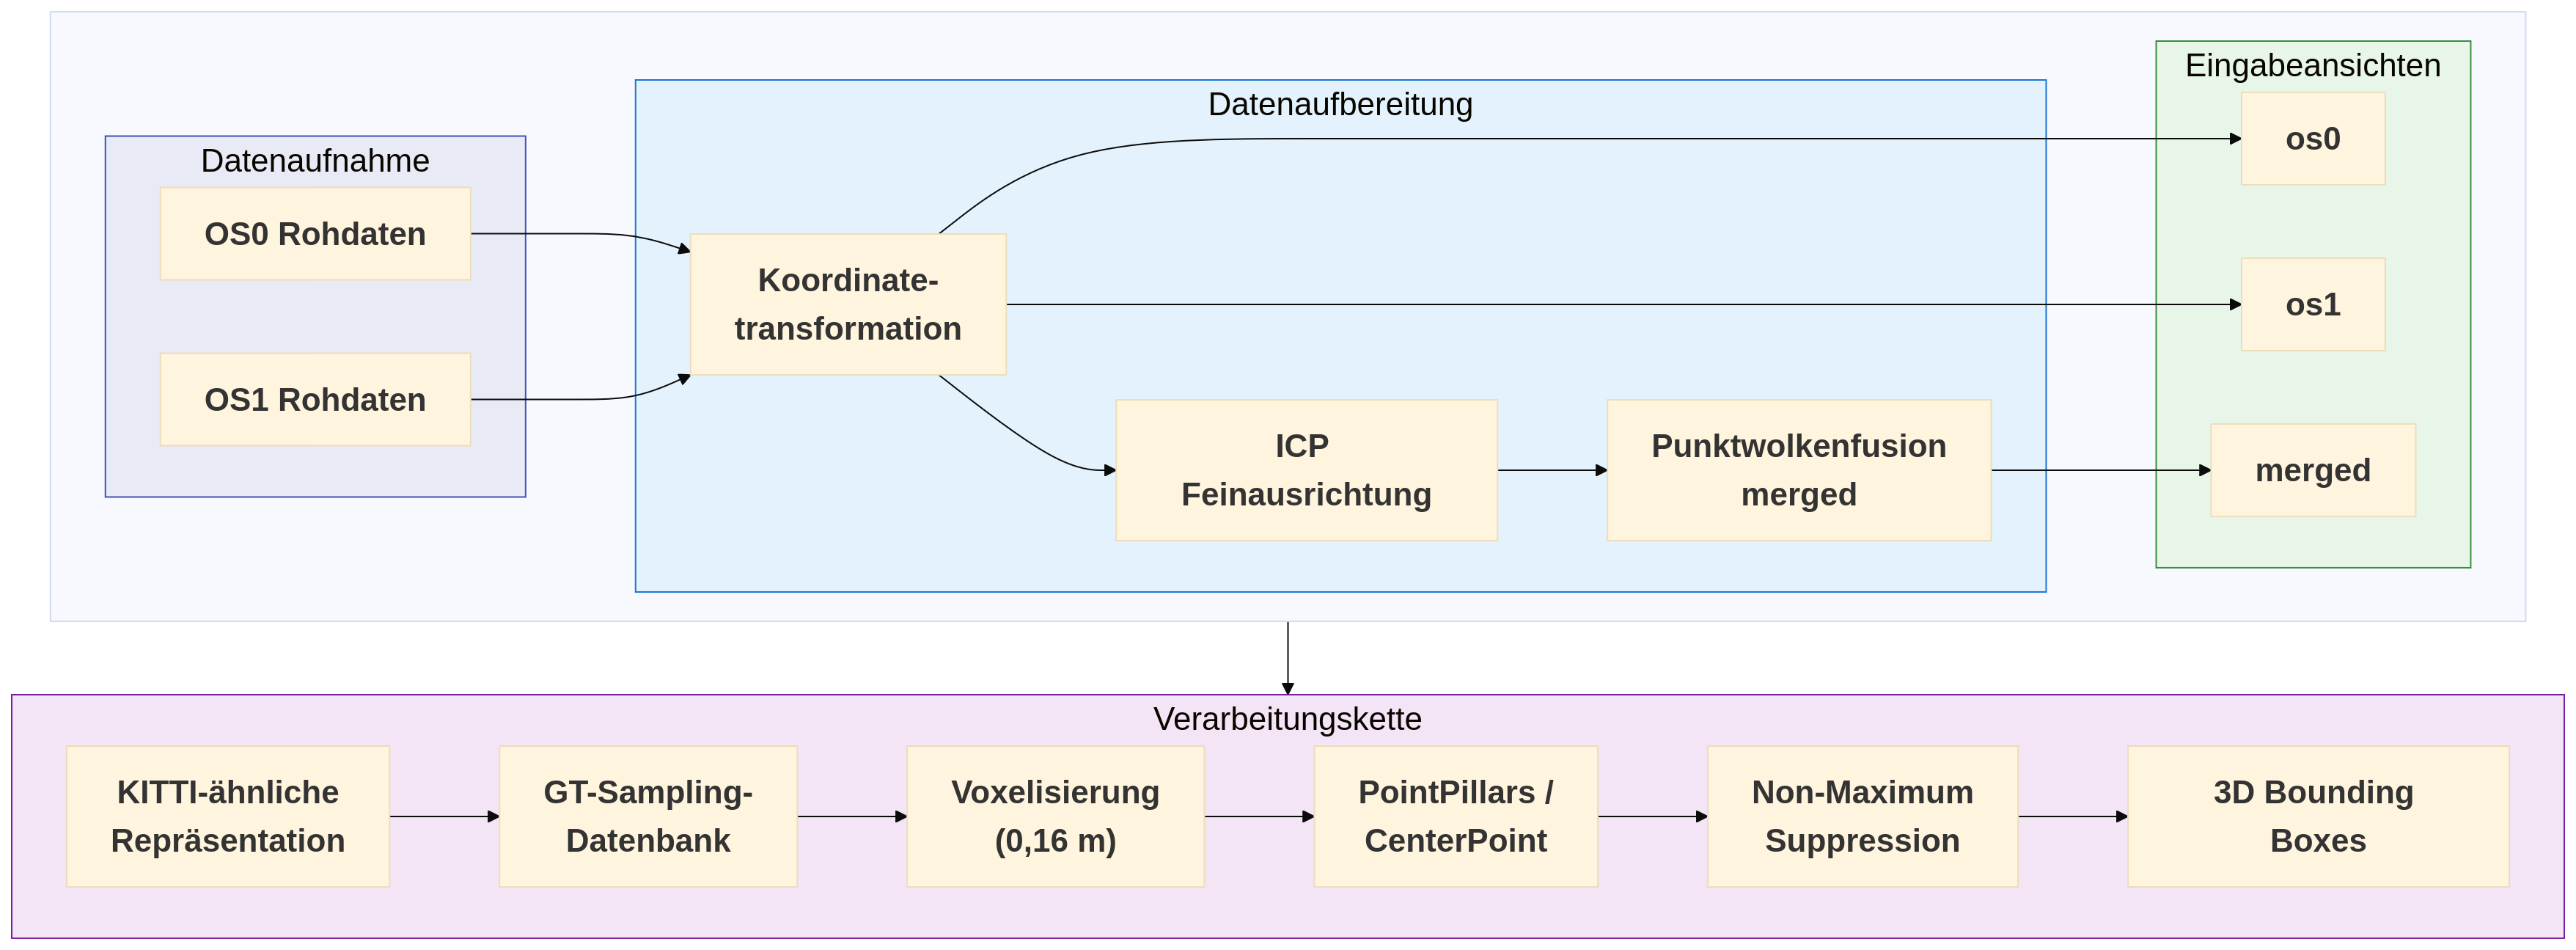
\includegraphics[width=\textwidth]{images/pipeline-diagram.png}
\caption{Verarbeitungskette von den Rohdaten über Fusion und Augmentierung bis zur 3D-Box-Prädiktion.}
\label{fig:pipeline}
\end{figure}

\subsection{Registrierung und Merge}

Die Merge-Pipeline ist in \texttt{experiment/pcd\_merge.py} implementiert. Sie führt für jedes Sensorpaar folgende Schritte aus:

\begin{enumerate}
    \item Laden der beiden Punktwolken und ihrer Intensitätswerte,
    \item Entfernen statistischer Ausreißer,
    \item Anwenden einer manuell bestimmten Vorabtransformation,
    \item Voxel-Downsampling und Normalenschätzung,
    \item Feinausrichtung durch Iterative Closest Point (ICP) \cite{besl1992icp},
    \item Konkatenation der transformierten Punkte.
\end{enumerate}

Die beiden Sensoren sind fest montiert. Für einen späteren Online-Betrieb wäre deshalb eine einmalig auf einer geeigneten statischen Szene bestimmte Extrinsik vorzuziehen. Die aktuelle Implementierung berechnet die ICP-Korrektur dagegen für jeden Frame neu. Das ist für die Offline-Erzeugung der Projektdaten verwendbar, aber weder laufzeitoptimal noch als endgültige Live-Pipeline zu verstehen.

\subsection{Konvertierung in das Trainingsformat}
\label{sec:konvertierung}

MMDetection3D \cite{mmdet3d2020} verarbeitet die Daten in einer KITTI-ähnlichen Repräsentation \cite{geiger2012kitti}. Eigene Converter übertragen Punktwolken und Labels in dieses Format und erzeugen die benötigten Info-PKLs. Dabei wurden mehrere geometrische und metrische Fehler identifiziert und korrigiert:

\begin{itemize}
    \item \textbf{Abgeschnittener Boden.} Der Boden lag durch eine fehlerhafte \(z\)-Transformation außerhalb des vorgesehenen Punktwolkenbereichs. Dem Training fehlten dadurch der Boden und die unteren rund 40\,cm aller Objekte.
    \item \textbf{Schwebende Boxen.} Der Label-Editor speichert die \(z\)-Koordinate im Boxzentrum, während die Trainingspipeline an einer Stelle die Boxunterkante erwartete. Ohne Korrektur saßen die Boxen um eine halbe Objekthöhe, also ungefähr 75\,cm, zu hoch.
    \item \textbf{Nicht vergleichbare Intensitäten.} Intensitäten wurden ursprünglich frameabhängig normiert, sodass dieselbe Oberfläche je Aufnahme andere Werte erhielt. Sie werden nun mit einer festen Skala verarbeitet.
    \item \textbf{Verzerrte Metrik.} Die frühere Metrik mittelte AP pro Frame und wertete Frames ohne Instanz der betrachteten Klasse als Null. Da Fahrräder nur in einem Teil der Frames vorkommen, war die erreichbare Fahrrad-AP dadurch nach oben gedeckelt. Die aktuelle Implementierung berechnet datensatzweite AP.
\end{itemize}

Der Metrikfehler war der folgenreichste der vier Punkte, weil er nicht das Modell, sondern dessen Bewertung betraf: Auf identischem Modelloutput steigt der Fahrrad-AP\textsubscript{30} von 0{,}24 auf 0{,}94, sobald datensatzweit statt frameweise gemittelt wird. Aufgefallen ist der Fehler, weil zwei unterschiedlich trainierte Modelle exakt denselben Fahrradwert erreichten -- genau das Maximum, das die fehlerhafte Rechnung überhaupt zulässt. Das fehlerhafte Vorgehen hat die Modellqualität also nie verschlechtert, sondern nur verdeckt.

Alle in diesem Bericht genannten Leistungszahlen basieren auf dem korrigierten Datenstand. Frühere absolute Werte, die mit abgeschnittenem Boden, verschobenen Boxen oder der fehlerhaften Pro-Frame-Metrik entstanden sind, wurden verworfen und werden nicht berichtet.

Davon zu unterscheiden sind die in den Abschnitten~\ref{sec:gtsampling} und \ref{sec:ursachen} herangezogenen Ablationen. Sie stammen aus einer früheren Projektphase und dienen ausschließlich dem relativen Vergleich zweier Konfigurationen, die jeweils unter identischen Bedingungen trainiert wurden. Ihre Richtungsaussagen werden hier verwendet, ihre absoluten Werte nicht. Auf welchem Datenstand die Ablationen im Einzelnen gelaufen sind, ist im Bericht nicht durchgängig dokumentiert; eine Wiederholung auf dem korrigierten Stand steht aus.

\newpage
\section{Modelle und Training}

\subsection{PointPillars}

PointPillars \cite{lang2019pointpillars} wandelt die unregelmäßige Punktwolke in ein Raster senkrechter Säulen, sogenannter Pillars, um. Innerhalb jedes Pillars werden die Punkte zu einem Merkmalsvektor verdichtet. Anschließend verarbeitet ein zweidimensionales Backbone die entstehende Bird's-Eye-View-Repräsentation und sagt orientierte 3D-Boxen voraus.

Das Modell wird nicht von Grund auf neu trainiert. Ausgangspunkt ist ein auf KITTI \cite{geiger2012kitti} vortrainierter Drei-Klassen-Checkpoint. Dieses Vorwissen wird durch Finetuning auf die Tiefgaragenszene angepasst \cite{pan2010transfer}. Für jeden Fold und jede Ansicht wird ein eigenes Modell trainiert. Insgesamt entstehen damit neun evaluierbare PointPillars-Foldmodelle.

Die wesentlichen Trainingsparameter sind in Tabelle~\ref{tab:training-params} zusammengefasst:

\begin{table}[H]
\centering
\begin{tabular}{ll}
\toprule
\textbf{Parameter} & \textbf{Festgelegter Wert} \\
\midrule
Initialisierung & KITTI-Drei-Klassen-Checkpoint \\
Trainingsdauer & 50 Epochen \\
Optimierer & AdamW, \(\beta = (0{,}95;\ 0{,}99)\), Weight Decay 0{,}01 \\
Lernrate & \(1 \cdot 10^{-4}\), zyklischer Zeitplan \\
Batchgröße & 6 pro GPU \\
Punktwolkenbereich & \([0;\ 69{,}12] \times [-39{,}68;\ 39{,}68] \times [-3;\ 1]\,\text{m}\) \\
Pillargröße & \(0{,}16 \times 0{,}16 \times 4\,\text{m}\) \\
Zufallsseed & 42 \\
Klassen & Person, Fahrrad, Auto \\
Checkpoint-Auswahl & höchste Validierungs-mAP \\
GT-Sampling & Person 8, Fahrrad 10 \\
\bottomrule
\end{tabular}
\caption{Festgelegte Trainingsparameter für PointPillars. Die GT-Sampling-Werte geben an, wie viele Instanzen der jeweiligen Klasse pro Trainingsframe maximal zusätzlich eingefügt werden.}
\label{tab:training-params}
\end{table}

Für jede Fold-/Ansichtskombination wird die GT-Sampling-Datenbasis ausschließlich aus deren Trainingsframes erzeugt. Test- und Validierungsobjekte können daher nicht durch Copy-Paste-Augmentierung in das Training gelangen.

\subsection{Klassenungleichgewicht und GT-Sampling}
\label{sec:gtsampling}

In den Trainingsdaten kommen deutlich mehr Autos als Fahrräder vor; im früheren \texttt{merged}-Trainingssplit lag das Verhältnis ungefähr bei 22:1. GT-Sampling fügt zusätzliche Personen- und Fahrradinstanzen aus anderen Trainingsframes in die aktuelle Trainingsszene ein \cite{ghiasi2021copypaste}. Dadurch steigt die Variabilität der seltenen Klassen, ohne Frames aus Validierung oder Test zu verwenden.

Frühere kontrollierte Ablationen zeigten, dass GT-Sampling die Fahrrad-Detektion verbessert. Einfaches Frame-Oversampling war weniger wirksam. Diese Ablationen stammen aus einer früheren Projektphase; herangezogen wird ausschließlich ihre Richtungsaussage, nicht ihr absolutes Niveau (Abschnitt~\ref{sec:konvertierung}). Ein Filter für Punkte unterhalb des Bodens reduzierte die Fehldetektionen nicht und verschlechterte andere Ergebnisse; er wurde deshalb nicht in die Standardpipeline übernommen.

\subsection{Architekturvergleich mit CenterPoint}
\label{sec:architekturvergleich}

Zusätzlich wurde CenterPoint \cite{yin2021centerpoint} unter dem in Abschnitt~\ref{sec:evalprotokoll} beschriebenen Cross-Validation-Protokoll trainiert. CenterPoint ist im Gegensatz zum anchorbasierten PointPillars ein anchorfreier Detektor, der Objektzentren über eine Heatmap vorhersagt.

Der Vergleich verfolgt eine einzige Frage: Hängt der Fusionsbefund an der gewählten Architektur, oder gilt er auch für einen anders aufgebauten Detektor? Er dient damit als Robustheitsprüfung der Modellwahl und ausdrücklich nicht als nachträgliche Optimierung des Testprotokolls. Beide Modelle wurden unter demselben Cross-Validation-Protokoll mit denselben Folds und denselben Ansichten trainiert und ausgewertet.

Die Vorgehensweise ist für beide Architekturen identisch. Übereinstimmend sind Trainingsdauer, Zufallsseed, Klassensatz, Initialisierung aus einem auf KITTI vortrainierten Checkpoint, Augmentierung einschließlich GT-Sampling sowie die Checkpoint-Auswahl nach höchster Validierungs-mAP; es gelten also die in Tabelle~\ref{tab:training-params} festgelegten Werte. Unterschiedlich sind ausschließlich die Detektorarchitektur und die untrennbar an sie gebundenen Einstellungen, etwa der Aufbau des Detektionskopfes und die ankerbasierte gegenüber der ankerfreien Zuordnung. Diese wurden für beide Modelle aus der jeweiligen Referenzkonfiguration übernommen und nicht auf die Projektdaten abgestimmt; keines der beiden Modelle erhielt damit einen gezielten projektspezifischen Tuningvorteil.

Damit ist nicht nur die Rangfolge der Ansichten innerhalb jeder Architektur vergleichbar, sondern auch der absolute Abstand zwischen den beiden Modellen ein kontrollierter Vergleich der beiden verwendeten Referenzkonfigurationen auf diesem Datensatz. Die verwendete PointPillars-Konfiguration erzielt in allen Ansichten höhere Werte und bleibt daher das Hauptmodell dieser Arbeit.

\newpage
\section{Evaluationsprotokoll}
\label{sec:evalprotokoll}

\subsection{Warum der frühere temporale Split ersetzt wurde}

Die erste Auswertung verwendete innerhalb jedes Experiments eine zeitliche 80/10/10-Aufteilung. Im Fall der Autoaufnahmen lagen die Testframes damit am Ende der Trajektorie. Splitzugehörigkeit und Objektposition waren gekoppelt.

Konkret hatte das bewegte Auto in den letzten zehn Prozent der Aufnahme den gut einsehbaren Bereich bereits verlassen. Das Testsegment enthielt das Zielobjekt also kaum noch oder nur stark verdeckt. Der sehr niedrige damalige dynamische Auto-AP\textsubscript{30} von \(\texttt{os1}=0{,}09\) beschrieb somit nicht die allgemeine Qualität von \texttt{os1}, sondern die Generalisierung auf diesen letzten räumlichen Trajektorienabschnitt.

Dieser Befund darf nicht mehr als Hauptresultat verwendet werden. Die Cross-Validation mit vollständig zurückgehaltenen Experimenten ersetzt den temporalen Split als wissenschaftliche Hauptbewertung.

\subsection{Experiment-held-out Cross-Validation}

Das Protokoll wurde am 11. Juli 2026 vor der Sichtung der Cross-Validation-Testergebnisse eingefroren \cite{raschka2018model}. Abbildung~\ref{fig:cv-fold-diagramm} gibt einen Überblick über das Schema.

\begin{figure}[H]
\centering
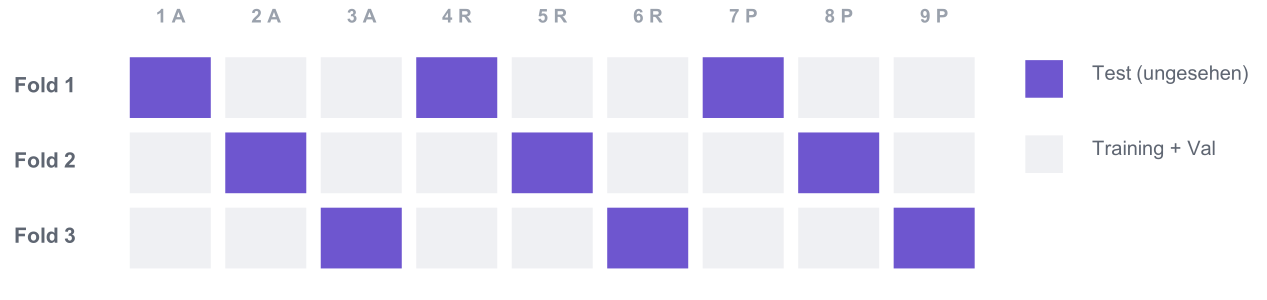
\includegraphics[width=\textwidth]{images/cv-fold-diagramm.png}
\caption[Schema der experiment-held-out Cross-Validation]{Experiment-held-out Cross-Validation: Jedes Experiment wird in genau einem Fold getestet, die übrigen dienen mit einem zeitlichen Guard dem Training und der Validierung.}
\label{fig:cv-fold-diagramm}
\end{figure}

Die drei Folds sind in Tabelle~\ref{tab:cv-folds} zusammengefasst:

\begin{table}[H]
\centering
\begin{tabular}{cc}
\toprule
\textbf{Fold} & \textbf{Vollständig ungesehene Testexperimente} \\
\midrule
1 & Auto~1, Fahrrad~4, Person~7 \\
2 & Auto~2, Fahrrad~5, Person~8 \\
3 & Auto~3, Fahrrad~6, Person~9 \\
\bottomrule
\end{tabular}
\caption{Experiment-held-out Cross-Validation: Zusammensetzung der drei Folds.}
\label{tab:cv-folds}
\end{table}

Innerhalb der jeweils übrigen sechs Experimente werden die letzten zehn Prozent als Validierungsdaten verwendet. Die zehn davorliegenden Frames pro Trainingsexperiment werden als zeitlicher Guard ausgeschlossen. Die vollständigen Testexperimente werden weder für das Training noch für die Checkpoint-Auswahl verwendet. Tabelle~\ref{tab:cv-split-counts} gibt die resultierenden Frame-Anzahlen pro Fold wieder.

\begin{table}[H]
\centering
\begin{tabular}{ccccc}
\toprule
\textbf{Fold} & \textbf{Training} & \textbf{Validierung} & \textbf{Test} & \textbf{Guard} \\
\midrule
1 & 1.239 & 146 & 677 & 60 \\
2 & 1.172 & 137 & 753 & 60 \\
3 & 1.227 & 143 & 692 & 60 \\
\bottomrule
\end{tabular}
\caption{Frame-Anzahlen pro Fold nach Training, Validierung, Test und Guard.}
\label{tab:cv-split-counts}
\end{table}

Alle drei Ansichten erhalten pro Fold identische physische Zeitstempel. Damit ist der View-Vergleich zeitlich gepaart. Die bereits erwähnten ansichtsspezifischen Labels bleiben jedoch erhalten.

\subsection{Metriken}

Eine Vorhersage gilt als Treffer, wenn ihre dreidimensionale Intersection over Union (IoU) mit einer noch nicht zugeordneten Ground-Truth-Box derselben Klasse den betrachteten Schwellwert erreicht. Verwendet werden AP\textsubscript{30}, AP\textsubscript{40}, AP\textsubscript{50} und AP\textsubscript{60}:

\begin{itemize}
    \item AP\textsubscript{30} bewertet überwiegend, ob das Objekt ungefähr gefunden wurde.
    \item AP\textsubscript{60} verlangt eine deutlich präzisere räumliche Lokalisierung.
    \item Der Klassen-mAP mittelt über AP\textsubscript{30} bis AP\textsubscript{60}.
    \item Der Gesamt-mAP mittelt zusätzlich über die drei Klassen.
\end{itemize}

Die tiefgestellten Zahlen bezeichnen durchgehend die IoU-Schwelle in Prozent. Die AP selbst wird als datensatzweite, elfpunktinterpolierte AP berechnet. Vorhersagen werden nach ihrem Konfidenzscore sortiert; Matching bleibt frameweise, die Precision-Recall-Kurve wird jedoch aus der gesamten Testmenge aufgebaut.

\subsection{Fold-Mittel und gepoolte Out-of-Fold-Auswertung}

Die Fold-Ergebnisse sind die primäre Generalisierungsschätzung. Aus ihnen werden Mittelwert und Stichproben-Standardabweichung berechnet. Zusätzlich werden die Vorhersagen aller drei Testfolds zu einer gepoolten Out-of-Fold-Auswertung zusammengeführt. Dabei wurde jeder Frame genau von dem Modell vorhergesagt, für das sein vollständiges Experiment ungesehen war.

Die gepoolte AP wird einmal auf der gemeinsamen Rangliste aller Out-of-Fold-Vorhersagen berechnet. Sie ist deshalb nicht identisch mit dem arithmetischen Mittel dreier AP-Werte. Da die Konfidenzscores der drei Foldmodelle unterschiedlich kalibriert sein können, ergänzt der gepoolte Wert die Foldanalyse, ersetzt sie aber nicht.

\subsection{Offizielle und labelbasierte Auswertung bewegter Objekte}

Die offizielle dynamische Teilbewertung ignoriert eine Vorhersage auf einem statischen Objekt nur, wenn diese am jeweiligen Evaluationsschwellwert ausreichend mit der statischen GT-Box überlappt. Eine etwas ungenau lokalisierte, aber eindeutig einem geparkten Auto zuordenbare Box kann dadurch bei AP\textsubscript{60} als False Positive der dynamischen Rangliste erscheinen.

Deshalb existiert zusätzlich eine benannte labelbasierte Variante. Sie nutzt das manuelle \texttt{static}-Attribut und ignoriert Vorhersagen auf Nichtzielobjekten bereits ab IoU 0{,}25. Die regulären All-Object-Metriken bleiben dabei bit-identisch; nur die Teilranglisten für bewegte und statische Objekte ändern sich. Die offizielle Auswertung bleibt die Vergleichsreferenz, während die labelbasierte Variante die interpretierbare Analyse der bewegten Objekte liefert.

Zur Offenlegung gehört, wie diese Variante entstanden ist. Sie wurde nicht gemeinsam mit dem Cross-Validation-Protokoll eingefroren, sondern erst nach der Analyse des in Abschnitt~\ref{sec:ap60-artefakt} beschriebenen AP\textsubscript{60}-Artefakts definiert. Ihre Wirkung fällt zugunsten der fusionierten Ansicht aus und zeigt damit in Richtung der untersuchten Hypothese. Aus diesem Grund gelten drei Festlegungen: Die offizielle Auswertung bleibt unverändert dokumentiert und behält den Status der Vergleichsreferenz, jede Angabe aus der labelbasierten Variante wird als solche gekennzeichnet, und die Regel wird für alle drei Ansichten identisch angewendet. Alle zentralen Ergebnisse werden deshalb unter beiden Varianten berichtet (Tabellen~\ref{tab:bewegt-fold} und \ref{tab:alle-schwellen}). Im aggregierten Bewegt-mAP bleibt die Rangfolge der Ansichten in beiden Varianten dieselbe. Auf der Ebene einzelner Klassen und Schwellen können sich Werte und Rangfolge dagegen unterscheiden; am deutlichsten beim bewegten Auto, wo die offizielle Variante \texttt{os0} vorn sieht und die labelbasierte \texttt{merged}. Beim Fahrrad sind beide Varianten identisch, weil in den Daten keine statischen Fahrräder annotiert sind.

\newpage
\section{Ergebnisse}

\subsection{Wirkung des Finetunings}
\label{sec:finetuning-wirkung}

Die erste Forschungsfrage betrifft den Nutzen des Finetunings gegenüber einem unverändert übernommenen vortrainierten Modell. Die Vorgängerarbeit \cite{pagel2025railway} hat auf denselben Aufnahmen mehrere ausschließlich vortrainierte Modelle ohne Anpassung an die Zielszene ausgewertet. Abbildung~\ref{fig:finetuning-baseline} stellt diese Werte dem hier erreichten Fold-Mittel gegenüber.

\begin{figure}[H]
\centering
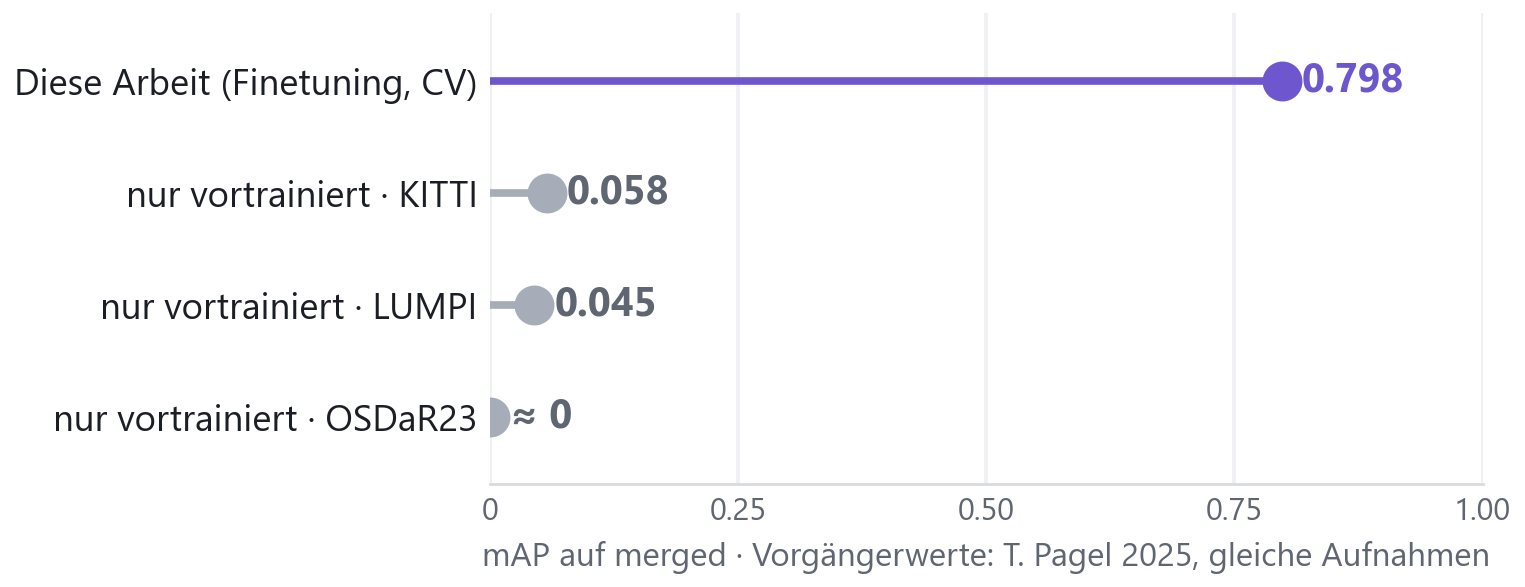
\includegraphics[width=0.9\textwidth]{images/finetuning-baseline.png}
\caption[Finetuning gegenüber vortrainierten Modellen]{Gesamt-mAP auf der fusionierten Ansicht: Finetuning in dieser Arbeit gegenüber ausschließlich vortrainierten Modellen. Die Vergleichswerte stammen aus \cite{pagel2025railway} und wurden auf denselben Tiefgaragenaufnahmen erhoben, aus denen auch Abbildung~\ref{fig:setup} übernommen ist; der Titel jener Arbeit verweist auf einen weiteren, hier nicht betrachteten Anwendungsfall.}
\label{fig:finetuning-baseline}
\end{figure}

Ohne Anpassung an die Zielszene bleiben die vortrainierten Modelle bei einem mAP von 0{,}058 (KITTI), 0{,}045 (LUMPI) beziehungsweise nahe null (OSDaR23). Das in dieser Arbeit auf den Projektdaten finetunete PointPillars erreicht 0{,}798. Der Abstand beträgt damit 0{,}740 mAP; das finetunete Modell erreicht einen ungefähr 14-mal so hohen Wert.

Diese Gegenüberstellung ist ausdrücklich ein Größenordnungsvergleich und keine kontrollierte Ablation. Die Vergleichswerte stammen aus einer anderen Arbeit und wurden nicht unter dem hier verwendeten Cross-Validation-Protokoll erhoben; identisch sind lediglich die zugrunde liegenden Aufnahmen. Insbesondere ist nicht bekannt, ob dort dieselbe Datenkonvertierung und dieselbe AP-Berechnung verwendet wurden. Wie folgenreich das sein kann, zeigt Abschnitt~\ref{sec:konvertierung}: Allein der Wechsel von einer frameweisen auf eine datensatzweite Mittelung veränderte den Fahrrad-AP\textsubscript{30} bei identischem Modelloutput von 0{,}24 auf 0{,}94. Der hier genannte Abstand von 0{,}740 mAP ist deshalb keine quantitativ bestimmte Wirkung des Finetunings. Die Richtung der Aussage ist bei einem Unterschied dieser Größe dennoch eindeutig: Ein direkt übernommenes, auf Außenverkehrsdaten vortrainiertes Netz ist auf dieser Tiefgaragenszene praktisch unbrauchbar. Der Schritt auf die Zieldaten ist der entscheidende Hebel, nicht die Wahl der Architektur -- ein Befund, den der Architekturvergleich in Abschnitt~\ref{sec:centerpoint-ergebnis} stützt.

\subsection{Gesamtleistung von PointPillars}
\label{sec:gesamtleistung}

\begin{table}[H]
\centering
\begin{tabular}{ccccc}
\toprule
\textbf{Ansicht} & \textbf{Fold 1} & \textbf{Fold 2} & \textbf{Fold 3} & \textbf{Mittel \(\pm\) Std.} \\
\midrule
merged & 0{,}840 & 0{,}786 & 0{,}768 & \(0{,}798 \pm 0{,}037\) \\
os0    & 0{,}793 & 0{,}781 & 0{,}757 & \(0{,}777 \pm 0{,}018\) \\
os1    & 0{,}801 & 0{,}751 & 0{,}759 & \(0{,}770 \pm 0{,}027\) \\
\bottomrule
\end{tabular}
\caption{PointPillars Gesamt-mAP über alle Objekte: Fold-Werte, Mittel und Standardabweichung.}
\label{tab:pp-mAP-overall}
\end{table}

Wie Tabelle~\ref{tab:pp-mAP-overall} zeigt, erzielt \texttt{merged} in jedem Fold den höchsten Gesamt-mAP. Der mittlere Vorsprung beträgt ungefähr 0{,}021 gegenüber \texttt{os0} und 0{,}028 gegenüber \texttt{os1}. Bei nur drei Folds ist das kein starker Signifikanznachweis. Es ist jedoch ein konsistenter Hinweis darauf, dass Fusion die ausgewogenste Gesamtleistung liefert und in keinem Fold von einer Einzelsicht übertroffen wird.

Dieser Wert umfasst alle annotierten Objekte, also auch die zahlreichen geparkten Fahrzeuge, die über viele Aufnahmen hinweg an denselben Positionen stehen. Der Gesamt-mAP bewertet damit zwei verschiedene Fähigkeiten zugleich: die Generalisierung auf bewegte Zielobjekte und die Wiedererkennung statischer Szenenbestandteile. Wie stark sich der zweite Anteil auf die einzelnen Ansichten auswirkt, lässt sich aus den vorliegenden Zahlen nicht auftrennen, da die AP keine mengengewichtete Mittelung ist und der statische Anteil sich deshalb nicht herausrechnen lässt. Der folgende Abschnitt wertet die bewegten Objekte separat aus; dort fällt der Abstand zwischen den Ansichten deutlich größer aus.

\subsection{Bewegte Objekte: Gesamtbild}
\label{sec:bewegte-gesamt}

Beschränkt man den mAP auf die bewegten Zielobjekte, vergrößert sich der Abstand deutlich (Abbildung~\ref{fig:map-bewegt}):

\begin{figure}[H]
\centering
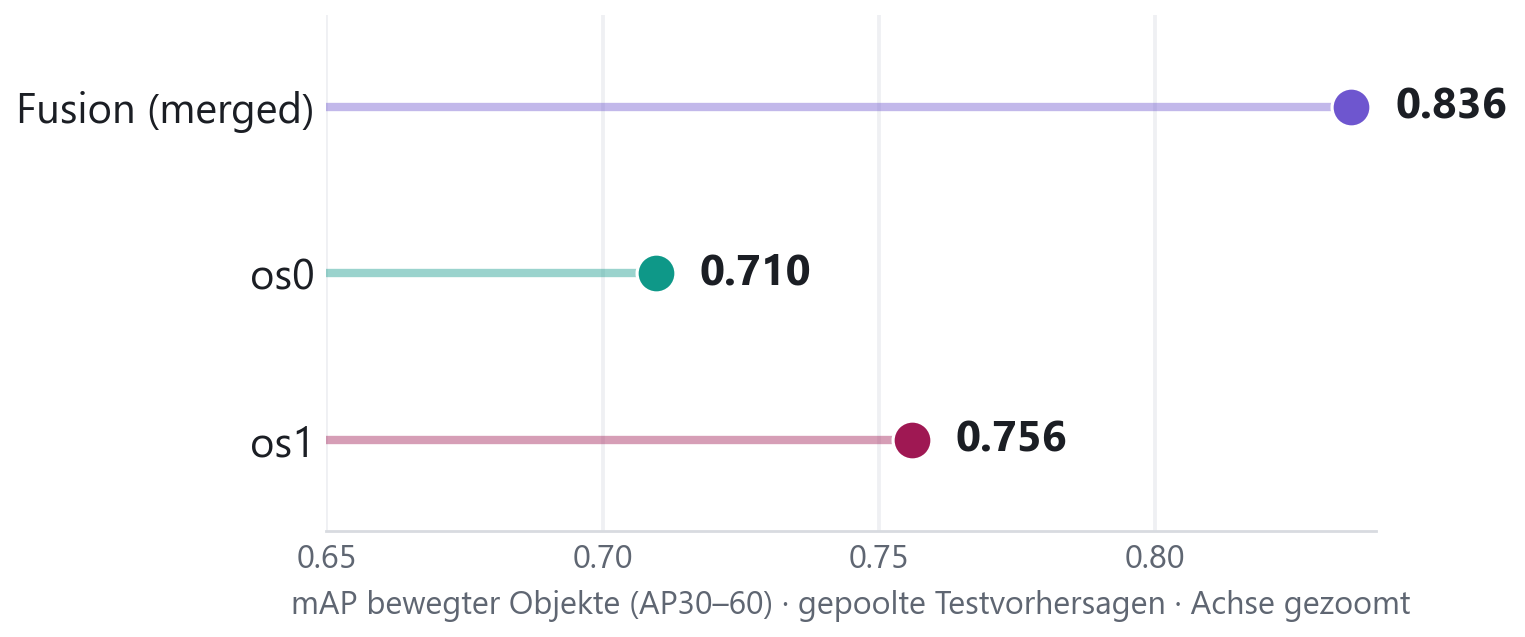
\includegraphics[width=0.9\textwidth]{images/map-bewegte-objekte.png}
\caption[mAP der bewegten Objekte je Ansicht]{mAP über AP\textsubscript{30} bis AP\textsubscript{60} und die drei Klassen, ausschließlich für bewegte Objekte (gepoolte Out-of-Fold-Vorhersagen, labelbasierte Bewegt-/Statisch-Variante).}
\label{fig:map-bewegt}
\end{figure}

Damit der Vergleich mit dem Gesamt-mAP des vorigen Abschnitts nicht zwei verschiedene Schätzer gegenüberstellt, gibt Tabelle~\ref{tab:bewegt-fold} den Bewegt-mAP ebenfalls als Fold-Mittel mit Stichproben-Standardabweichung an, und zwar unter beiden Auswertungsvarianten.

\begin{table}[H]
\centering
\begin{tabular}{cccc}
\toprule
\textbf{Ansicht} & \textbf{alle Objekte} & \textbf{bewegt, offiziell} & \textbf{bewegt, labelbasiert} \\
\midrule
merged & \(0{,}798 \pm 0{,}037\) & \(0{,}784 \pm 0{,}060\) & \(0{,}832 \pm 0{,}038\) \\
os0    & \(0{,}777 \pm 0{,}018\) & \(0{,}736 \pm 0{,}037\) & \(0{,}746 \pm 0{,}031\) \\
os1    & \(0{,}770 \pm 0{,}027\) & \(0{,}744 \pm 0{,}049\) & \(0{,}763 \pm 0{,}049\) \\
\bottomrule
\end{tabular}
\caption{mAP im Fold-Mittel: über alle Objekte sowie ausschließlich über bewegte Objekte, jeweils unter der offiziellen und der labelbasierten Variante.}
\label{tab:bewegt-fold}
\end{table}

Auf einheitlicher Grundlage wächst der Vorsprung der Fusion gegenüber der besseren Einzelansicht von 0{,}021 über alle Objekte auf 0{,}040 in der offiziellen und 0{,}069 in der labelbasierten Bewegt-Auswertung. Die Richtung ist damit in beiden Varianten dieselbe, und der Vergleich ist nun ein Vergleich gleichartiger Schätzer. Die gepoolten Werte in Abbildung~\ref{fig:map-bewegt} liegen mit 0{,}836, 0{,}756 und 0{,}710 nahe an den labelbasierten Fold-Mitteln.

Zwei Beobachtungen ergänzen das Bild. Erstens ist die Fusion in der Bewegt-Auswertung nicht die streuungsärmste Ansicht: Unter der offiziellen Variante liegt ihre Fold-Standardabweichung mit 0{,}060 über der von \texttt{os0} und \texttt{os1}. Zweitens kehrt sich die Reihenfolge der beiden Einzelsensoren um: Über alle Objekte liegt \texttt{os0} vorn, auf den bewegten Objekten \texttt{os1}. Der Unterschied zwischen beiden ist mit 0{,}008 beziehungsweise 0{,}017 allerdings klein gegenüber ihrer Fold-Streuung und sollte nicht als gesicherte Rangfolge gelesen werden.

\subsection{Bewegte Objekte nach Klasse}
\label{sec:bewegte-klassen}

Tabelle~\ref{tab:moving-objects-ap} und Abbildung~\ref{fig:ap30-ap60} schlüsseln dasselbe Ergebnis nach Klasse und IoU-Schwelle auf:

\begin{table}[H]
\centering
{\small\setlength{\tabcolsep}{4pt}
\begin{tabular}{cccc}
\toprule
\textbf{Ansicht} & \textbf{Person AP\textsubscript{30}/AP\textsubscript{60}} & \textbf{Fahrrad AP\textsubscript{30}/AP\textsubscript{60}} & \textbf{Auto AP\textsubscript{30}/AP\textsubscript{60}} \\
\midrule
merged & 0{,}901 / 0{,}729 & 0{,}800 / 0{,}668 & 0{,}891 / 0{,}883 \\
os0    & 0{,}653 / 0{,}370 & 0{,}895 / 0{,}378 & 0{,}885 / 0{,}856 \\
os1    & 0{,}896 / 0{,}426 & 0{,}744 / 0{,}529 & 0{,}832 / 0{,}789 \\
\bottomrule
\end{tabular}}
\caption{Labelbasierte AP\textsubscript{30}/AP\textsubscript{60} für bewegte Objekte nach Ansicht und Klasse (gepoolte OOF-Auswertung).}
\label{tab:moving-objects-ap}
\end{table}

\begin{figure}[H]
\centering
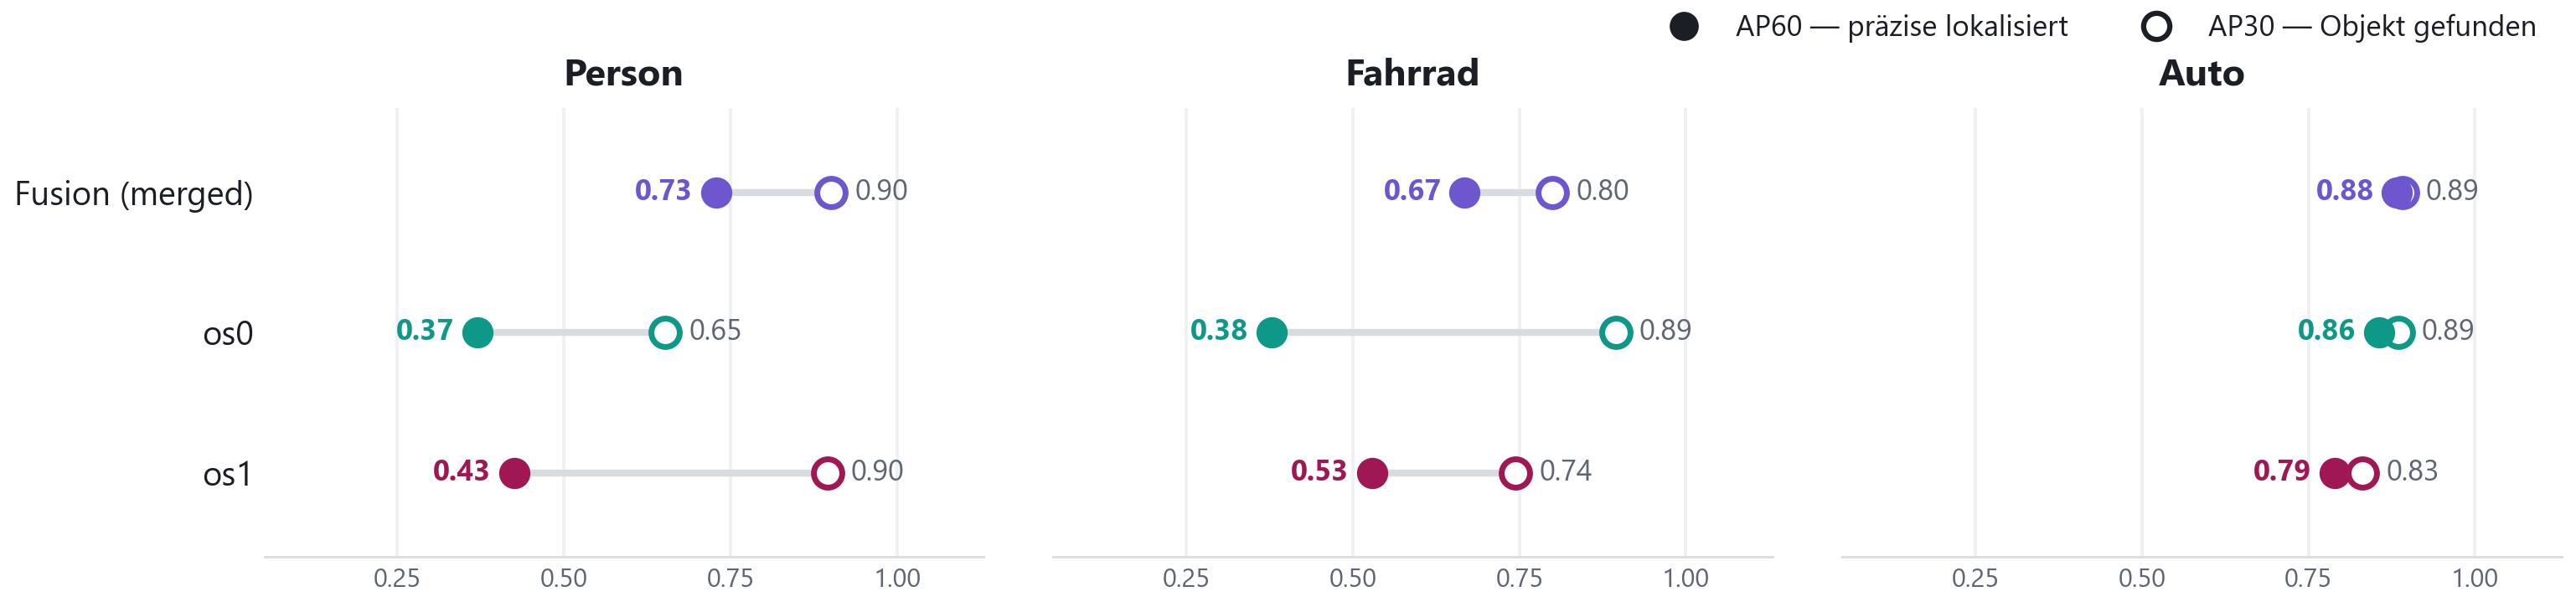
\includegraphics[width=\textwidth]{images/ap30-ap60-klassen.png}
\caption[Detektion gegenüber Lokalisierung je Klasse]{Detektion (AP\textsubscript{30}, offene Ringe) gegenüber präziser Lokalisierung (AP\textsubscript{60}, gefüllte Punkte) je Klasse und Ansicht. Der Abstand zwischen Ring und Punkt visualisiert den AP-Rückgang beim Übergang zur strengeren IoU-Schwelle und damit die Empfindlichkeit gegenüber höheren Lokalisierungsanforderungen. Er ist kein Anteil einzelner Objekte, da die AP über die gesamte Precision-Recall-Kurve gebildet wird.}
\label{fig:ap30-ap60}
\end{figure}

Die Darstellung trennt zwei Aspekte:

\begin{itemize}
    \item Bei AP\textsubscript{30} liegen alle Ansichten bei mindestens 0{,}65 und überwiegend über 0{,}80. Grundsätzlich wird also jede bewegte Klasse aus jeder Ansicht gefunden.
    \item Bei AP\textsubscript{60} liegt \texttt{merged} in allen drei Klassen vorn, bei Person und Fahrrad mit deutlichem Abstand. Der Fusionsvorteil zeigt sich damit in der räumlichen Präzision und nicht im Finden an sich.
\end{itemize}

Tabelle~\ref{tab:alle-schwellen} führt alle vier Schwellen auf, über die der mAP mittelt, und stellt beide Auswertungsvarianten gegenüber.

\begin{table}[H]
\centering
{\small\setlength{\tabcolsep}{4pt}
\begin{tabular}{llcccccccc}
\toprule
& & \multicolumn{4}{c}{\textbf{offiziell}} & \multicolumn{4}{c}{\textbf{labelbasiert}} \\
\cmidrule(lr){3-6}\cmidrule(lr){7-10}
\textbf{Ansicht} & \textbf{Klasse} & AP\textsubscript{30} & AP\textsubscript{40} & AP\textsubscript{50} & AP\textsubscript{60} & AP\textsubscript{30} & AP\textsubscript{40} & AP\textsubscript{50} & AP\textsubscript{60} \\
\midrule
merged & Person  & 0{,}901 & 0{,}899 & 0{,}796 & 0{,}561 & 0{,}901 & 0{,}900 & 0{,}879 & 0{,}729 \\
       & Fahrrad & 0{,}800 & 0{,}800 & 0{,}793 & 0{,}668 & 0{,}800 & 0{,}800 & 0{,}793 & 0{,}668 \\
       & Auto    & 0{,}877 & 0{,}750 & 0{,}739 & 0{,}739 & 0{,}891 & 0{,}891 & 0{,}891 & 0{,}883 \\
\midrule
os0    & Person  & 0{,}653 & 0{,}650 & 0{,}558 & 0{,}284 & 0{,}653 & 0{,}650 & 0{,}574 & 0{,}370 \\
       & Fahrrad & 0{,}895 & 0{,}874 & 0{,}639 & 0{,}378 & 0{,}895 & 0{,}874 & 0{,}639 & 0{,}378 \\
       & Auto    & 0{,}885 & 0{,}885 & 0{,}855 & 0{,}847 & 0{,}885 & 0{,}885 & 0{,}857 & 0{,}856 \\
\midrule
os1    & Person  & 0{,}896 & 0{,}884 & 0{,}743 & 0{,}276 & 0{,}896 & 0{,}884 & 0{,}842 & 0{,}426 \\
       & Fahrrad & 0{,}744 & 0{,}744 & 0{,}732 & 0{,}529 & 0{,}744 & 0{,}744 & 0{,}732 & 0{,}529 \\
       & Auto    & 0{,}831 & 0{,}828 & 0{,}823 & 0{,}783 & 0{,}832 & 0{,}829 & 0{,}825 & 0{,}789 \\
\bottomrule
\end{tabular}}
\caption{Gepoolte AP der bewegten Objekte über alle vier Evaluationsschwellen, offizielle gegenüber labelbasierter Variante.}
\label{tab:alle-schwellen}
\end{table}

Daraus folgen drei Punkte:

\begin{itemize}
    \item \textbf{Die AP\textsubscript{60}-Führung von \texttt{merged} besteht auch offiziell.} Bei Person führt \texttt{merged} offiziell mit 0{,}561 gegenüber 0{,}284 und 0{,}276, bei Fahrrad mit 0{,}668 gegenüber 0{,}378 und 0{,}529. Beim Fahrrad sind beide Varianten sogar identisch, weil in den Daten keine statisch gelabelten Fahrräder vorkommen und die labelbasierte Regel dort nicht greifen kann. Nur beim Auto kehrt sich die Rangfolge um; die Ursache ist in Abschnitt~\ref{sec:ap60-artefakt} aufgeklärt.
    \item \textbf{Der Präzisionsverlust setzt spät ein.} Von AP\textsubscript{30} zu AP\textsubscript{40} verändern sich die Werte kaum; der Einbruch liegt überwiegend zwischen IoU 0{,}50 und 0{,}60. Die Modelle finden Objekte also nicht nur, sondern lokalisieren sie bis etwa IoU 0{,}5 stabil; erst darüber trennen sich die Ansichten.
    \item \textbf{Die Variantenwahl betrifft Person und Auto, das Fahrrad gar nicht.} Bei Person bleiben AP\textsubscript{30} und AP\textsubscript{40} unverändert; die Unterschiede treten erst bei AP\textsubscript{50} und AP\textsubscript{60} auf. Beim Auto wirkt sich die Variante dagegen bereits bei AP\textsubscript{30} geringfügig aus (\(+0{,}014\) für \texttt{merged}) und ab AP\textsubscript{40} deutlich (\(+0{,}141\)). Betroffen ist dabei fast ausschließlich \texttt{merged}; bei \texttt{os0} und \texttt{os1} bleiben die Autowerte bis auf höchstens 0{,}010 gleich. Das entspricht der Erklärung aus Abschnitt~\ref{sec:ap60-artefakt}, wonach die Ursache in Vorhersagen auf einem einzelnen geparkten Fahrzeug liegt, die nur in der fusionierten Ansicht in großer Zahl auftreten.
\end{itemize}

\subsection{Der Personen-Einbruch von os0}
\label{sec:os0-person}

Der auffälligste Wert der Tabelle ist der Personen-AP\textsubscript{30} von 0{,}653 bei \texttt{os0}, rund 0{,}25 unter \texttt{merged} und \texttt{os1}. Er ist kein Artefakt der gepoolten Auswertung, sondern in den einzelnen Folds vorhanden (Tabelle~\ref{tab:os0-person-folds}).

\begin{table}[H]
\centering
\begin{tabular}{ccccc}
\toprule
\textbf{Ansicht} & \textbf{Fold 1} & \textbf{Fold 2} & \textbf{Fold 3} & \textbf{Mittel \(\pm\) Std.} \\
\midrule
merged & 0{,}908 & 0{,}901 & 0{,}893 & \(0{,}901 \pm 0{,}007\) \\
os0    & 0{,}873 & 0{,}688 & 0{,}663 & \(0{,}742 \pm 0{,}114\) \\
os1    & 0{,}900 & 0{,}899 & 0{,}892 & \(0{,}897 \pm 0{,}004\) \\
\bottomrule
\end{tabular}
\caption{AP\textsubscript{30} für bewegte Personen je Fold. Der Einbruch von \texttt{os0} tritt in den Folds 2 und 3 auf und ist nicht auf die Poolung zurückzuführen.}
\label{tab:os0-person-folds}
\end{table}

Die Ursache lässt sich genau eingrenzen. In den Folds 2 und 3 enthält \texttt{os0} als bewegte Personen ausschließlich die Instanzen des jeweiligen Personen-Experiments: 314 in Fold 2 und 251 in Fold 3. Wertet man dieselben Instanzen allein auf den Frames ihres Experiments aus, erreicht \texttt{os0} 0{,}885 beziehungsweise 0{,}903 -- über die vollständige Testmenge des Folds dagegen nur 0{,}688 und 0{,}663. Die Ground-Truth-Menge ist in beiden Rechnungen identisch; unterschiedlich ist allein, welche Vorhersagen in die Rangliste eingehen.

Der Unterschied kann deshalb nur von Personen-Vorhersagen stammen, die \texttt{os0} in den Auto- und Fahrrad-Experimenten desselben Folds erzeugt, in denen keine bewegte Person vorhanden ist. Es handelt sich um echte Fehldetektionen, nicht um einen Kalibrierungseffekt zwischen den Foldmodellen. Dazu passt, dass \texttt{os0} mit 948 die mit Abstand meisten Personen-Geisterboxen aufweist (Abschnitt~\ref{sec:geisterboxen}).

Daraus folgt zugleich eine methodische Warnung für die experimentweise Auswertung des folgenden Abschnitts: Sie bewertet jede Ansicht nur auf den Frames, in denen die Zielklasse tatsächlich bewegt vorkommt, und übersieht systematisch Fehldetektionen außerhalb dieser Frames. Sie überschätzt damit Ansichten, die zu klassenfremden Fehlalarmen neigen -- im vorliegenden Fall \texttt{os0}.

\subsection{Generalisierung je Experiment}
\label{sec:generalisierung-experiment}

Die bisherigen Werte fassen über Experimente hinweg zusammen. Abbildung~\ref{fig:ap30-je-experiment} löst dieselbe Auswertung nach den neun ungesehenen Testexperimenten auf und ergibt 27 einzelne Bewertungen der jeweils bewegten Zielklasse.

\begin{figure}[H]
\centering
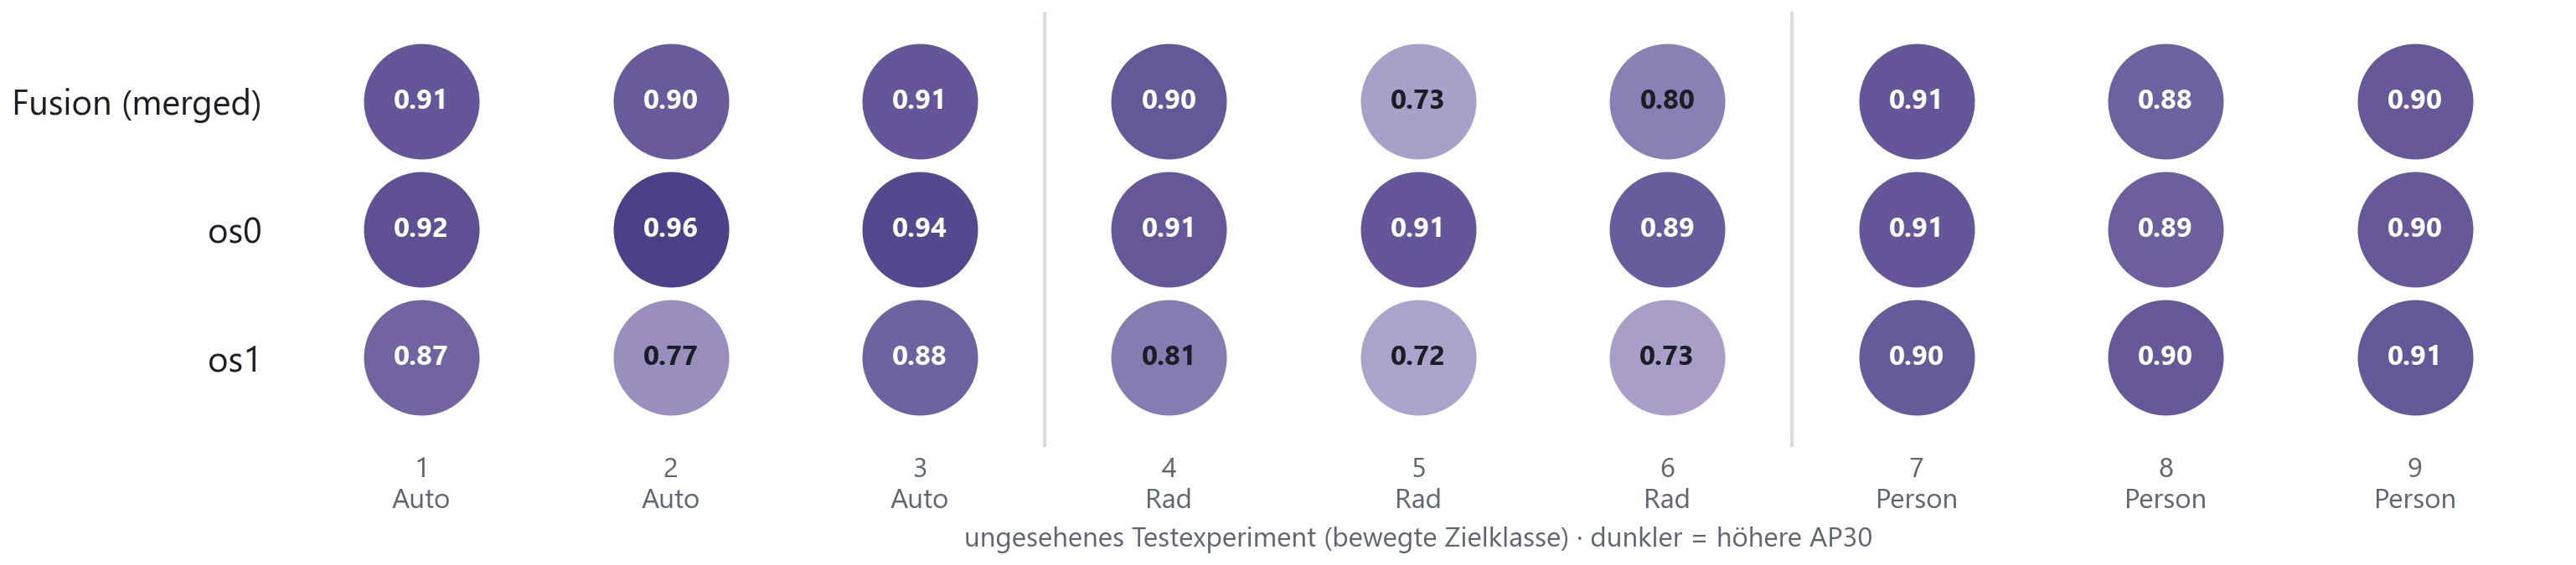
\includegraphics[width=\textwidth]{images/ap30-je-experiment.png}
\caption[AP\textsubscript{30} je ungesehenem Testexperiment]{AP\textsubscript{30} der bewegten Zielklasse je ungesehenem Testexperiment und Ansicht. Jede Spalte wurde von demjenigen Foldmodell vorhergesagt, für das dieses Experiment vollständig ungesehen war.}
\label{fig:ap30-je-experiment}
\end{figure}

Aus dieser Darstellung folgen drei Beobachtungen:

\begin{itemize}
    \item Es gibt keinen Ausfall. Der schlechteste Wert des gesamten Rasters beträgt 0{,}72 (\texttt{os1}, Fahrrad-Experiment 5). Der frühere Extremwert von 0{,}09 für \texttt{os1} auf dem bewegten Auto tritt unter dem Cross-Validation-Protokoll nicht mehr auf und war ein Artefakt des temporalen Splits.
    \item Beim bewegten Auto ist \texttt{os0} in allen drei Experimenten die stärkste Ansicht (0{,}92, 0{,}96 und 0{,}94). Die Fusion ist hier also nicht erforderlich, um das Auto zu finden. In der gepoolten Auswertung über alle Testframes dreht sich diese Ordnung knapp um (\texttt{merged} 0{,}891 gegenüber \texttt{os0} 0{,}885). Der Grund ist derselbe wie bei den Personen: Auch Autovorhersagen außerhalb der Autoaufnahmen gehen in die Rangliste ein. Welche Ansicht das bewegte Auto tatsächlich findet, beantwortet deshalb die experimentweise Auswertung; wie sich die Ansichten über den gesamten Betrieb hinweg verhalten, die gepoolte.
    \item Auf dieser Auswertung ist \texttt{os0} die stärkste und zugleich gleichmäßigste Ansicht. Über alle neun Experimente erreicht \texttt{os0} im Mittel 0{,}914 bei einer Standardabweichung von 0{,}023, \texttt{merged} 0{,}871 bei 0{,}063 und \texttt{os1} 0{,}832 bei 0{,}076. Die Fusion fällt im Fahrrad-Experiment 5 auf 0{,}73 ab und liegt in den Personen-Experimenten 8 und 9 knapp hinter \texttt{os1}.
\end{itemize}

Der letzte Punkt verdient Betonung, weil er der Fusionsthese zunächst widerspricht: Gemessen an der reinen Auffindrate über einzelne Experimente ist die Fusion nicht die beste Ansicht. Das ist kein Widerspruch zu den vorangegangenen Abschnitten, sondern eine Folge dessen, was dieses Raster misst. Es zeigt ausschließlich AP\textsubscript{30}, also die grobe Detektion. Der Vorteil der Fusion liegt nach Abschnitt~\ref{sec:bewegte-klassen} bei den strengeren Schwellen: Dort führt \texttt{merged} in der labelbasierten Auswertung in allen drei Klassen, bei Person und Fahrrad mit erheblichem Abstand. Ein vollständiges Bild ergäbe erst ein entsprechendes Raster für AP\textsubscript{60}, das bislang nicht vorliegt.

Zur Einordnung des Fahrrad-Experiments 5 siehe den folgenden Abschnitt; der dortige Sichtbarkeitseffekt erklärt den Abfall zu einem erheblichen Teil.

\subsection{Warum ist Fahrrad-\texorpdfstring{AP\textsubscript{30}}{AP30} bei os0 höher?}

\texttt{os0} erreicht bei Fahrrädern einen höheren AP\textsubscript{30}, während \texttt{merged} bei AP\textsubscript{60} deutlich führt. Ein Teil des AP\textsubscript{30}-Unterschieds ist ein Sichtbarkeits- und Label-Effekt. Die Ansichten enthalten nicht dieselbe Fahrrad-GT-Menge.

Besonders deutlich ist Experiment 5 (Tabelle~\ref{tab:exp5-bicycle}):

\begin{table}[H]
\centering
\begin{tabular}{ccc}
\toprule
\textbf{Ansicht} & \textbf{Fahrrad-GT} & \textbf{AP\textsubscript{30}} \\
\midrule
merged & 310 & 0{,}727 \\
os0    & 244 & 0{,}907 \\
\bottomrule
\end{tabular}
\caption{Experiment 5: Fahrrad-Ground-Truth-Anzahl und AP\textsubscript{30} nach Ansicht.}
\label{tab:exp5-bicycle}
\end{table}

In den Rohannotationen liegen die zusätzlichen \texttt{merged}-Fahrradframes gegenüber \texttt{os0} überwiegend weiter entfernt. \texttt{os0} wird damit teilweise nur auf dem kürzeren, gut sichtbaren Trajektorienabschnitt bewertet. Eine objektweise vollständig faire Aussage darüber, ob \texttt{merged} dieselben Fahrräder schlechter findet, würde eine zusätzliche Auswertung auf einer gemeinsamen Referenz-GT-Menge erfordern.

Unabhängig davon zeigt AP\textsubscript{60}, dass die von \texttt{merged} gefundenen Fahrräder räumlich wesentlich genauer lokalisiert werden. Die kurze Interpretation lautet daher: \texttt{os0} besitzt in seiner eigenen Labelmenge die vollständigere Groberkennung, die Fusion liefert die präziseren Boxen.

\subsection{Offizielle dynamische Auswertung und \texorpdfstring{AP\textsubscript{60}}{AP60}-Artefakt}
\label{sec:ap60-artefakt}

In der offiziellen dynamischen Auswertung beträgt der Auto-AP\textsubscript{30}/AP\textsubscript{60} \(0{,}877/0{,}739\) für \texttt{merged}, \(0{,}885/0{,}847\) für \texttt{os0} und \(0{,}831/0{,}783\) für \texttt{os1}. Der niedrige offizielle AP\textsubscript{60} von \texttt{merged} entsteht nicht primär durch eine schlechte Box auf dem bewegten Auto. Die beste \texttt{merged}-Box auf dem bewegten Auto hat im Median sogar die höchste IoU der drei Ansichten (\(0{,}848\)).

Der Haupttreiber ist ein nahe am Sensor geparktes Fahrzeug. Zahlreiche hochkonfidente \texttt{merged}-Vorhersagen liegen dort bei IoU 0{,}25--0{,}60. Sie werden bei der offiziellen AP\textsubscript{60}-Teilbewertung nicht mehr als statische Ignore-Treffer erkannt und erscheinen als False Positives in der dynamischen Rangliste. Die labelbasierte Variante ordnet diese Vorhersagen dem statischen Objekt zu; der \texttt{merged}-Auto-AP\textsubscript{60} steigt dadurch von 0{,}739 auf 0{,}883.

\subsection{Vergleich zu CenterPoint}
\label{sec:centerpoint-ergebnis}

Der in Abschnitt~\ref{sec:evalprotokoll} beschriebene Vergleich mit CenterPoint prüft, ob der Fusionsbefund an der gewählten Architektur hängt. Abbildung~\ref{fig:pp-vs-cp} zeigt die Fold-Mittel beider Modelle unter identischem Protokoll.

\begin{figure}[H]
\centering
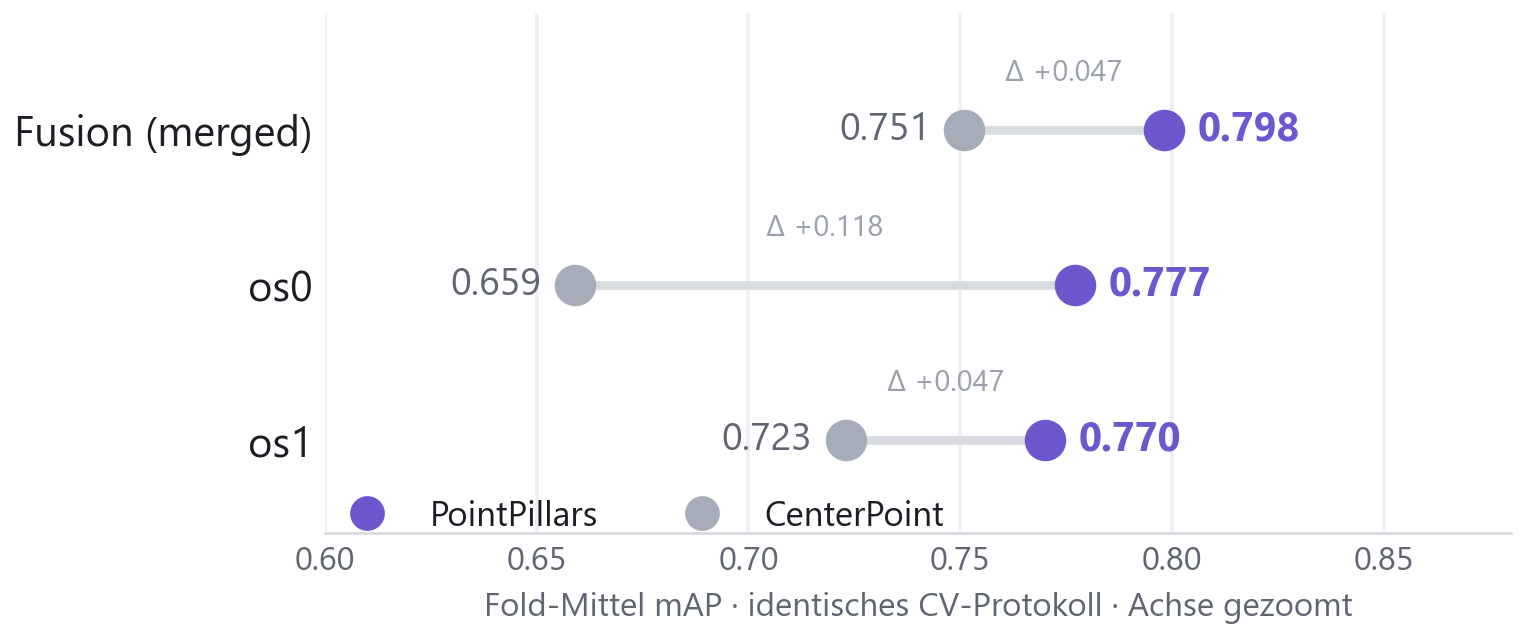
\includegraphics[width=0.9\textwidth]{images/pointpillars-vs-centerpoint.png}
\caption[PointPillars gegenüber CenterPoint]{Gesamt-mAP im Fold-Mittel: PointPillars gegenüber CenterPoint unter identischem Cross-Validation-Protokoll.}
\label{fig:pp-vs-cp}
\end{figure}

Das qualitative Ergebnis ist gegenüber dieser Alternativarchitektur robust: Auch bei CenterPoint ist \texttt{merged} in jedem Fold die beste Ansicht. Mit zwei getesteten Architekturen lässt sich zeigen, dass der Befund nicht ausschließlich an PointPillars hängt; eine allgemeine Architekturunabhängigkeit ist damit nicht belegt, zumal beide Modelle derselben gitterbasierten Detektorfamilie angehören. Die absolute Leistung liegt jedoch in allen drei Ansichten unter PointPillars, mit einem Abstand von 0{,}047 bis 0{,}118 mAP. Der Abstand entsteht vor allem durch die schwächere Lokalisierung von CenterPoint bei strengeren IoU-Schwellen, unter der labelbasierten dynamischen Auswertung besonders deutlich bei Fahrrädern.

Der Fusionsbefund hängt somit nicht an der anchorbasierten PointPillars-Architektur. Zusammen mit dem Ergebnis aus Abschnitt~\ref{sec:finetuning-wirkung} ergibt sich ein konsistentes Bild: Der Unterschied zwischen den Architekturen bewegt sich im Bereich von etwa 0{,}05 bis 0{,}12 mAP, der Unterschied zwischen vortrainiert und finetunet dagegen im Bereich von 0{,}74. Da beide Modelle in Trainingsprotokoll und Datengrundlage übereinstimmen und sich nur in der Architektur und den an sie gebundenen Einstellungen unterscheiden (Abschnitt~\ref{sec:architekturvergleich}), ist dieser Abstand auf den vorliegenden Daten kontrolliert gemessen. Auf eine allgemeine Überlegenheit von PointPillars gegenüber CenterPoint lässt er sich dennoch nicht verallgemeinern: Beide Modelle liefen in ihrer jeweiligen Referenzkonfiguration auf einer einzigen Szene, und ein gezielt auf diese Daten abgestimmtes CenterPoint könnte anders abschneiden. Für die weitere Ergebnisdiskussion bleibt PointPillars das Hauptmodell.

\newpage
\section{Qualitative Fehleranalyse}
\label{sec:fehleranalyse}

\subsection{Qualitativer Eindruck}

Abbildung~\ref{fig:bev-vergleich} zeigt denselben Frame einmal aus der Einzelsensoransicht \texttt{os1} und einmal aus der fusionierten Ansicht, jeweils in der Vogelperspektive mit Ground-Truth-Boxen und den Vorhersagen des zugehörigen Foldmodells.

\begin{figure}[H]
\centering
\begin{subfigure}{\textwidth}
\centering
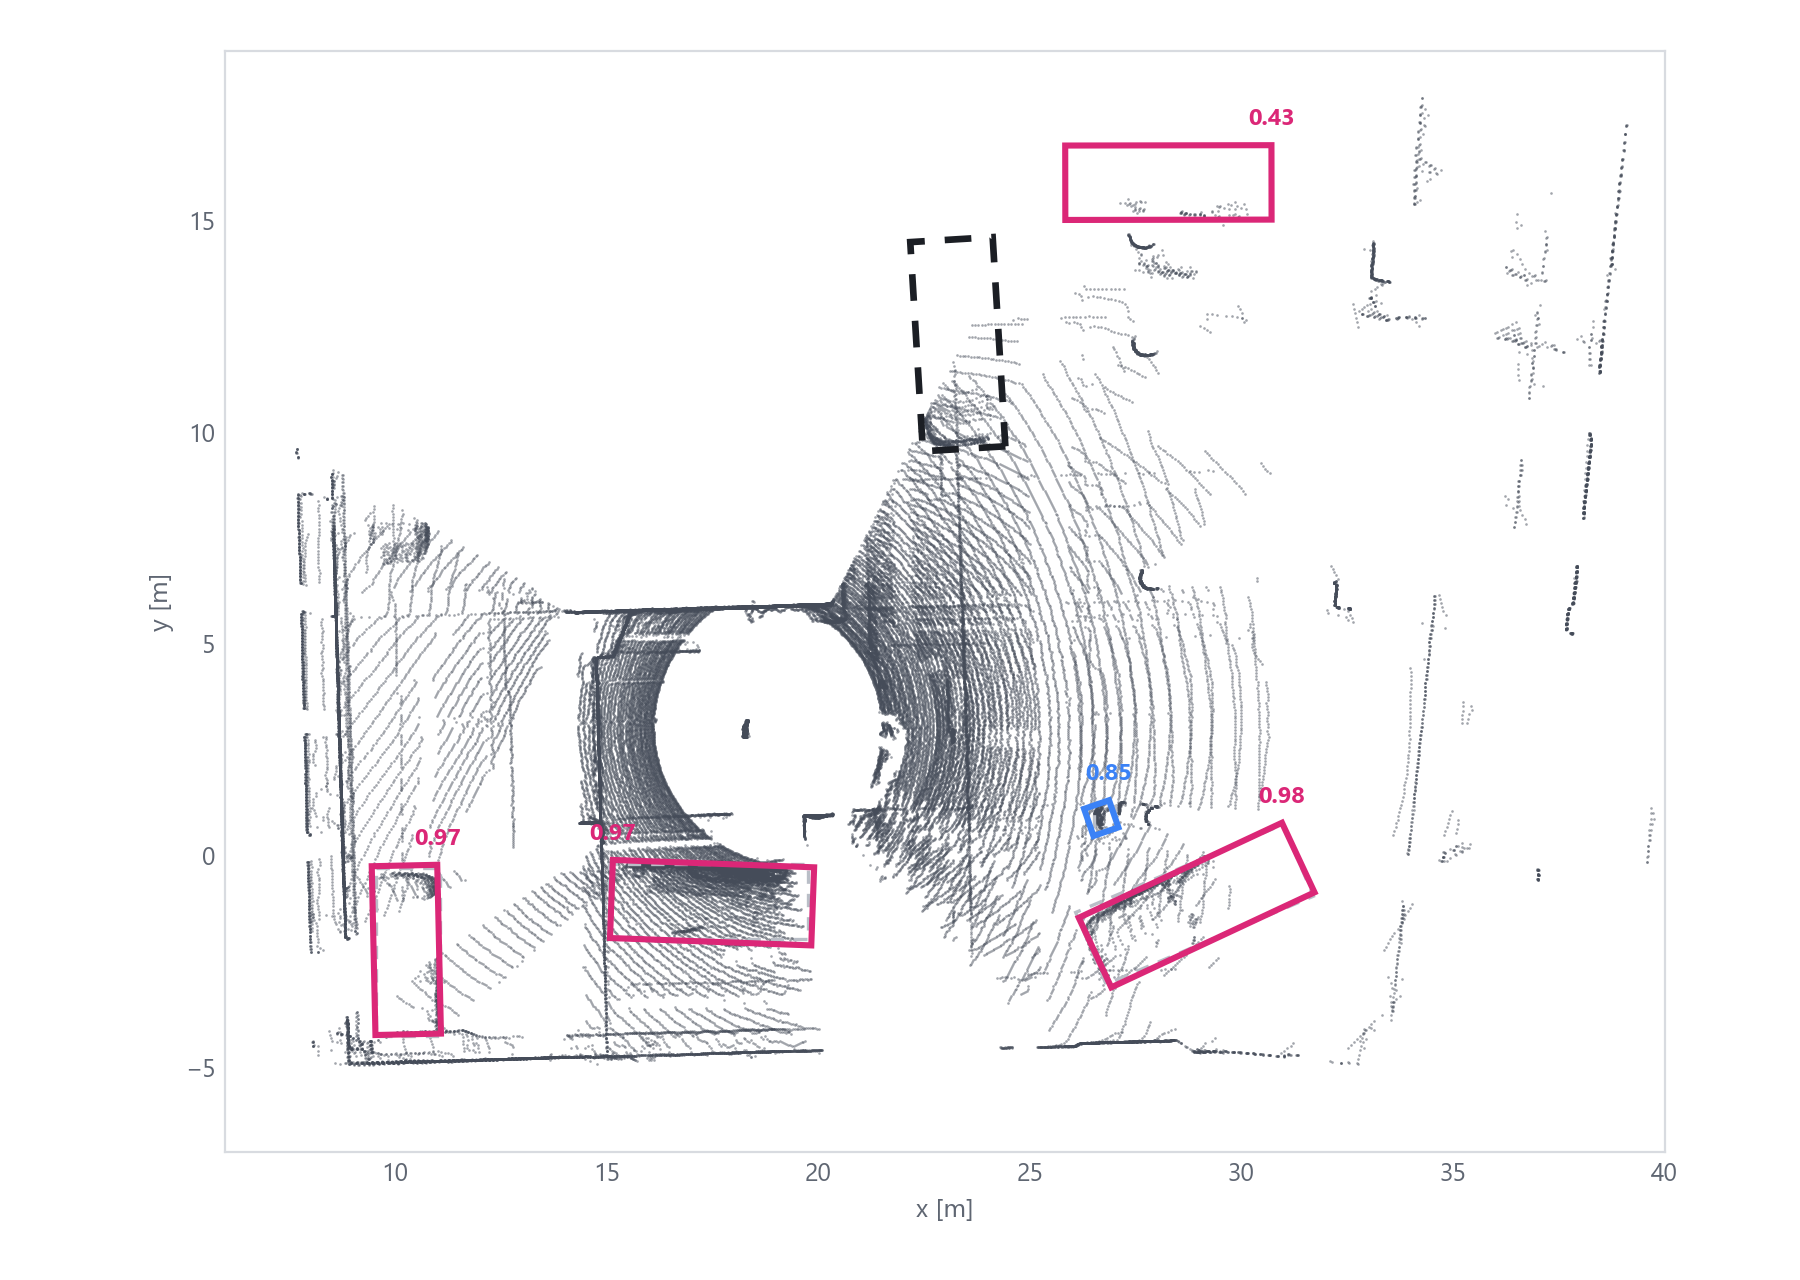
\includegraphics[width=0.62\textwidth]{images/bev-os1.png}
\caption{Einzelsensoransicht \texttt{os1}}
\label{fig:bev-einzel}
\end{subfigure}

\vspace{0.2cm}

\begin{subfigure}{\textwidth}
\centering
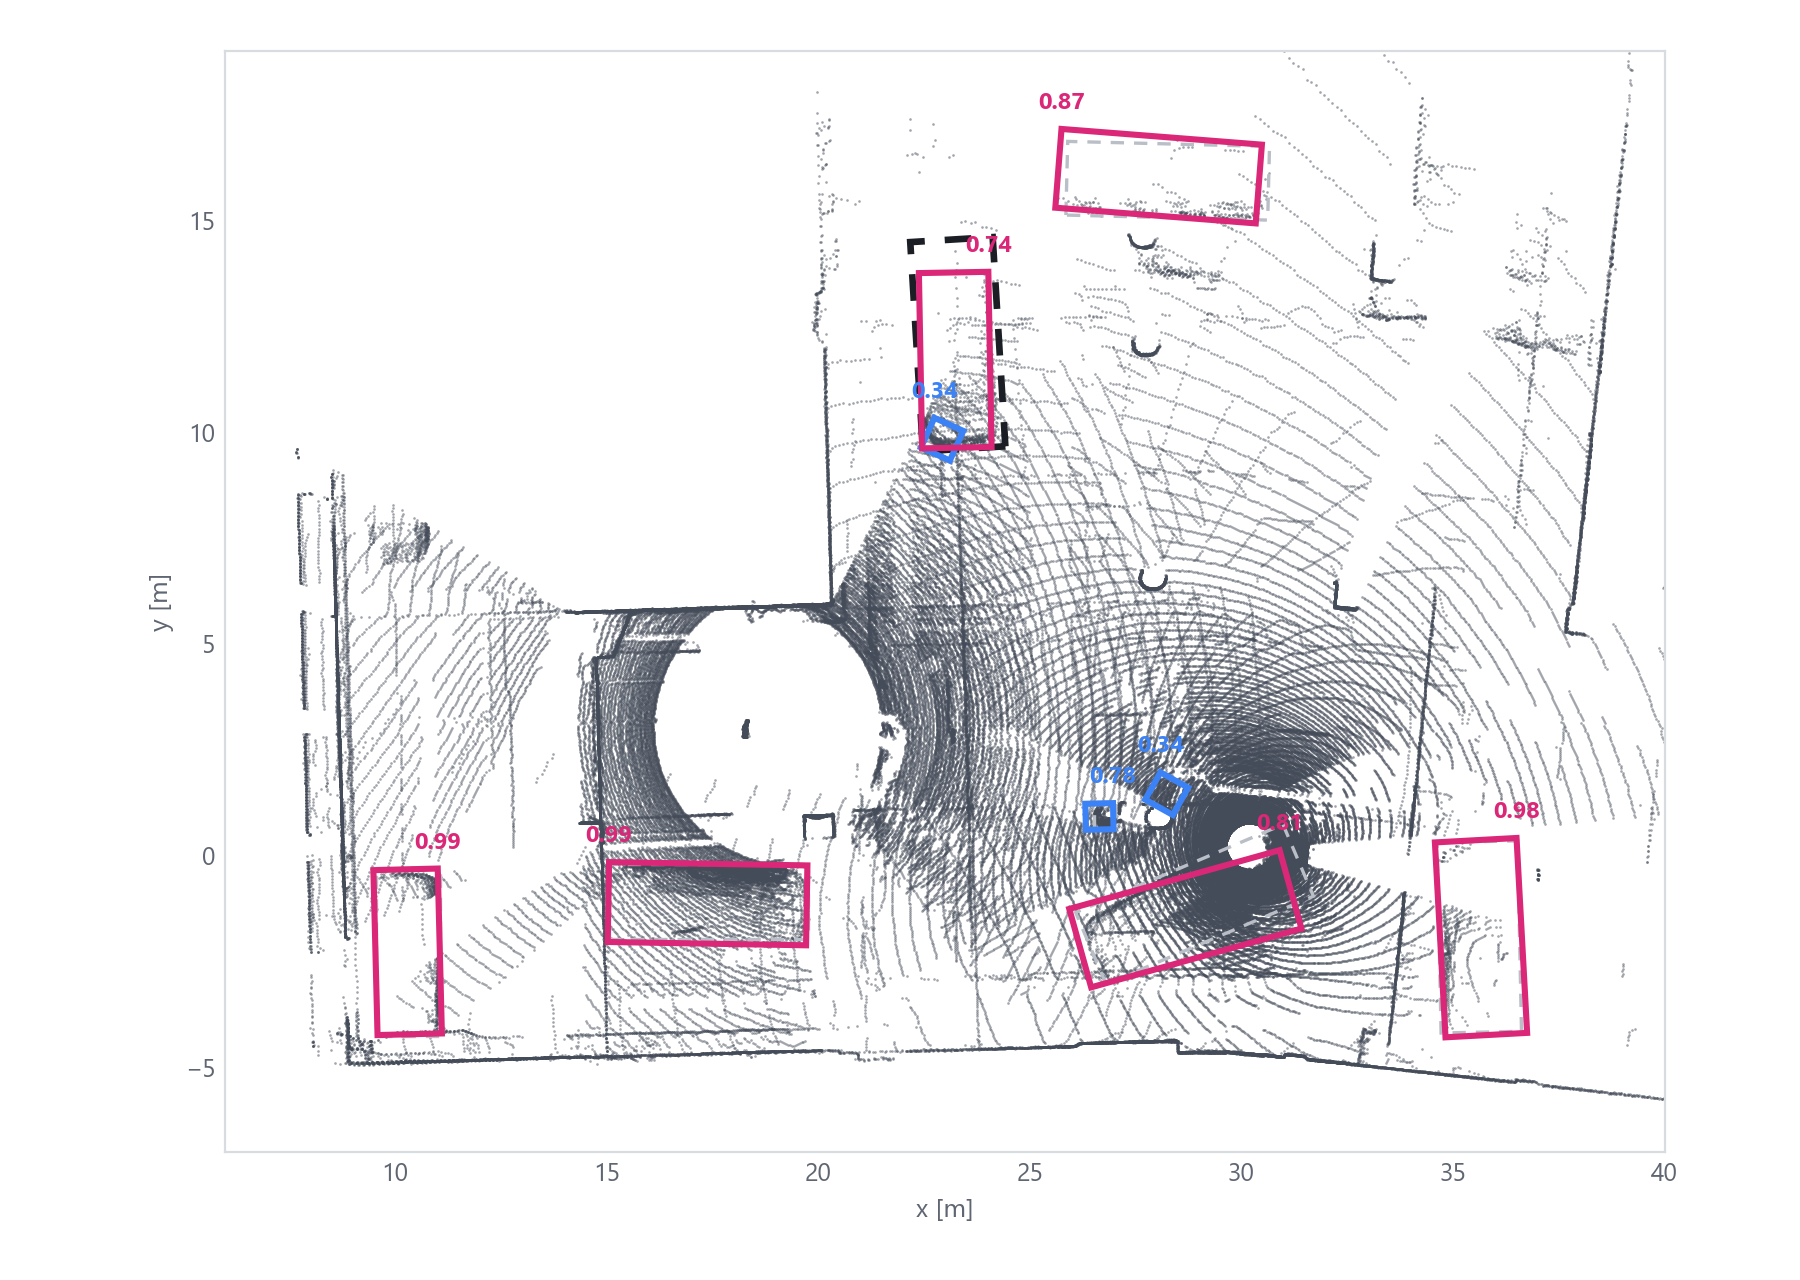
\includegraphics[width=0.62\textwidth]{images/bev-merged.png}
\caption{Fusionierte Ansicht \texttt{merged}}
\label{fig:bev-fusion}
\end{subfigure}
\caption{Derselbe Frame in Vogelperspektive. Gestrichelt: Ground Truth; durchgezogen mit Konfidenzwert: Vorhersagen. In~\subref{fig:bev-einzel} bleibt die gestrichelte Ground-Truth-Box des Autos im oberen Bildbereich ohne zugeordnete Vorhersage, weil das Fahrzeug aus der Perspektive von \texttt{os1} nur wenige Punkte erhält. In~\subref{fig:bev-fusion} ergänzen die Punkte von \texttt{os0} die verdeckte Fahrzeugseite, sodass dort eine Vorhersage entsteht.}
\label{fig:bev-vergleich}
\end{figure}

Das Bild illustriert den Mechanismus hinter dem Fusionsvorteil: Die zusätzliche Perspektive füllt Verdeckungen auf und erhöht die Punktdichte an Objektseiten, die aus einer einzelnen Richtung abgeschattet sind. Der gezeigte Einzelfall passt zum quantitativen Befund, denn \texttt{os1} erreicht beim Auto mit einem AP\textsubscript{30} von 0{,}832 den niedrigsten Wert der drei Ansichten (Tabelle~\ref{tab:moving-objects-ap}).

Zugleich zeigt die Abbildung die Grenze des Effekts, denn die in der fusionierten Ansicht entstehende Vorhersage besitzt nur eine geringe Konfidenz und würde eine übliche Betriebsschwelle nicht überschreiten. Einzelne Frames sind als Beleg ohnehin nicht ausreichend; die quantitative Grundlage bleibt die Cross-Validation.

\subsection{Definition der Geisterboxen}
\label{sec:geisterboxen}

Für die generalisierte OOF-Analyse wird eine Geisterbox als Vorhersage mit Score mindestens 0{,}3 definiert, die sich keiner noch unbenutzten GT-Box derselben Klasse bei 3D-IoU mindestens 0{,}3 zuordnen lässt. Diese Definition umfasst nicht nur leere Halluzinationen, sondern auch Duplikate, falsch klassifizierte reale Strukturen und schlecht lokalisierte Boxen.

Auf den 2.122 gemeinsamen Testframes ergeben sich die in Tabelle~\ref{tab:ghost-boxes} aufgeführten Geisterbox-Zahlen:

\begin{table}[H]
\centering
\begin{tabular}{ccccc}
\toprule
\textbf{Ansicht} & \textbf{Person} & \textbf{Fahrrad} & \textbf{Auto} & \textbf{Gesamt} \\
\midrule
merged & 510 & 315 & 159 & 984 \\
os0    & 948 & 157 & 415 & 1.520 \\
os1    & 329 & 372 & 248 & 949 \\
\bottomrule
\end{tabular}
\caption{Anzahl Geisterboxen (Score \(\geq\) 0{,}3, IoU \(<\) 0{,}3) auf den 2.122 gemeinsamen OOF-Testframes.}
\label{tab:ghost-boxes}
\end{table}

Abbildung~\ref{fig:geisterboxen-rate} normiert dieselben Zahlen auf 100 Frames und macht die Klassenzusammensetzung sichtbar.

\begin{figure}[H]
\centering
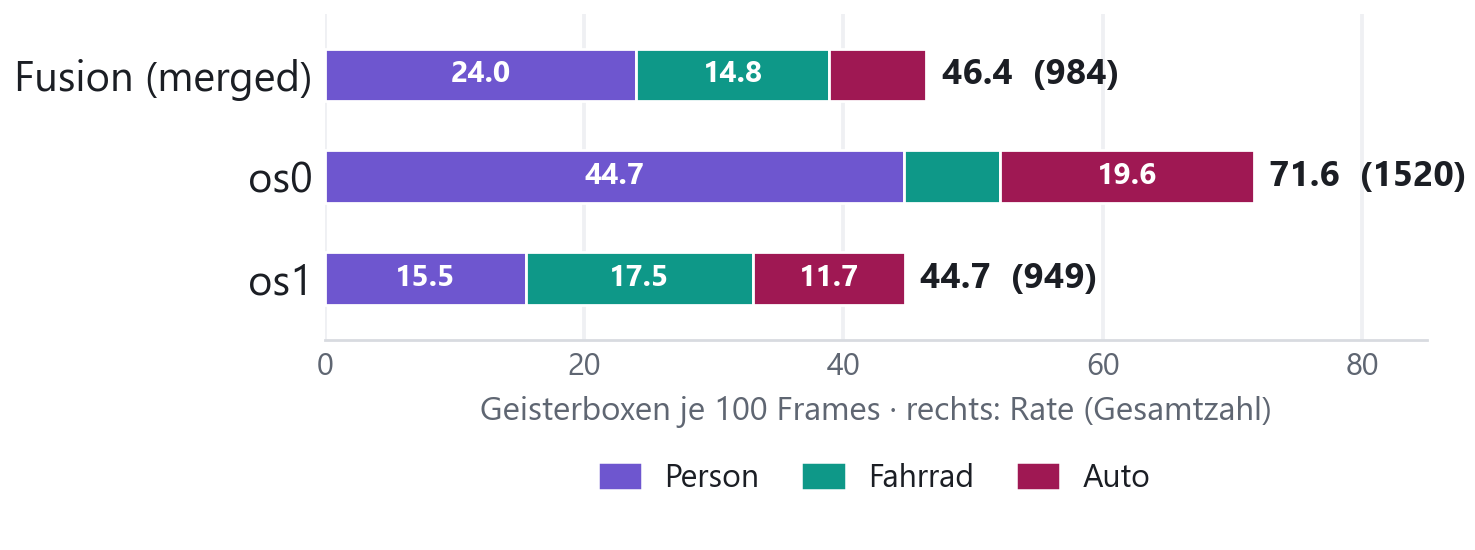
\includegraphics[width=0.95\textwidth]{images/geisterboxen-rate.png}
\caption{Geisterboxen je 100 Testframes, aufgeschlüsselt nach Klasse. Rechts die Gesamtrate mit der absoluten Anzahl in Klammern.}
\label{fig:geisterboxen-rate}
\end{figure}

Die Fehlerbilder unterscheiden sich deutlich zwischen den Ansichten. \texttt{os0} erzeugt mit 71{,}6 Geisterboxen je 100 Frames die mit Abstand höchste Rate, dominiert von Personen- und Autoboxen. \texttt{os1} und \texttt{merged} liegen mit 44{,}7 beziehungsweise 46{,}4 ähnlich, wobei bei \texttt{os1} die Fahrradboxen überwiegen. Die hohe Personen-Geisterboxrate von \texttt{os0} ist die unmittelbare Entsprechung des in Abschnitt~\ref{sec:os0-person} nachgewiesenen Personen-Einbruchs: Beide beschreiben dieselben Fehldetektionen, einmal als absolute Zahl und einmal in ihrer Wirkung auf die Precision-Recall-Kurve.

Dass \texttt{merged} trotz einer geringfügig höheren Rate als \texttt{os1} in allen mAP-Werten vorn liegt, ist kein Widerspruch. Die Geisterboxzählung ist eine absolute Fehlerzahl bei einer festen Konfidenzschwelle von 0{,}3 und keine Precision-Angabe. Die AP integriert dagegen über die gesamte Precision-Recall-Kurve und honoriert zusätzlich gefundene richtige Objekte. Die fusionierte Ansicht erzeugt mehr Vorhersagen insgesamt, darunter sowohl mehr Treffer als auch geringfügig mehr Fehldetektionen. Für den praktischen Betrieb bleibt die absolute Rate dennoch relevant, weil sie die Nachbearbeitung durch Tracking und Betriebsschwellen bestimmt.

\subsection{Plausible Ursachen}
\label{sec:ursachen}

Die detaillierte Fahrradforensik zeigt drei wiederkehrende Gruppen:

\begin{enumerate}
    \item Reale statische oder nicht gelabelte Strukturen werden als Fahrrad interpretiert.
    \item Sparse Reflexions- und Unterbodenpunkte können lokale Aktivierungen auslösen.
    \item Vorhersagen treten wiederholt an Positionen auf, an denen Fahrräder in den Trainingsaufnahmen vorkamen. Dies deutet auf eine ortsgebundene Szenenmemorierung hin.
\end{enumerate}

Ein Filter für Punkte unterhalb des Bodens reduzierte die Geisterboxen in einer Ablation nicht. Daraus folgt lediglich, dass Unterbodenpunkte allein den Effekt nicht erklären; Reflexionen, die oberhalb des Bodens entstehen, werden von dieser Ablation nicht erfasst und bleiben als Teilursache möglich.

Teilweise ragen Fahrrad- oder Personenboxen in die Ground-Truth-Box eines Autos. Das ist als klassenübergreifende Mehrfachhypothese plausibel: Dünn abgetastete Fahrzeugkanten oder das Heck können gleichzeitig einen fahrradähnlichen Anchor aktivieren. Die standardmäßige Non-Maximum Suppression arbeitet klassenweise. Eine korrekte Autobox unterdrückt deshalb keine zusätzliche Fahrradbox. Da die Zusatzbox keine Fahrrad-GT trifft, zählt sie in der Fahrradwertung als False Positive, auch wenn sie ein Auto überlappt.

Eine getestete Cross-Class-NMS entfernte vollständig enthaltene klassenübergreifende Zusatzboxen und veränderte die Metriken nicht. Sie ist als Ausgabebereinigung vertretbar, sollte aber nicht nachträglich anhand der Cross-Validation-Testdaten optimiert werden.

\subsection{Praktische Gegenmaßnahmen}

Für eine spätere Anwendung bieten sich folgende Maßnahmen an:

\begin{itemize}
    \item pro Klasse auf Validierungsdaten gewählte Konfidenzschwellen,
    \item zeitliche Trackbestätigung statt Entscheidungen aus einzelnen Frames,
    \item Hintergrundunterstützung oder eine statische Szenenkarte,
    \item Cross-Class-NMS als konservative Ausgabebereinigung,
    \item zusätzliche Trainingsszenen zur Verringerung der Ortsmemorierung.
\end{itemize}

\newpage
\section{Laufzeit}
\label{sec:laufzeit}

\subsection{Modellinferenz}

Die Laufzeiten wurden mit Batchgröße 1 auf einer Tesla V100-SXM3-32GB gemessen (Tabelle~\ref{tab:inference-runtime}). Die Messung umfasst die Modellpipeline einschließlich Datenverarbeitung und Voxelisierung auf bereits vorbereiteten Ansichtsdaten.

\begin{table}[H]
\centering
\begin{tabular}{cccc}
\toprule
\textbf{Ansicht} & \textbf{Durchsatz} & \textbf{Zeit pro Frame} & \textbf{Typische Punktzahl} \\
\midrule
merged & 11{,}7\,fps & 85\,ms & ca. 210.000 \\
os0    & 22{,}3\,fps & 45\,ms & ca. 105.000 \\
os1    & 23{,}5\,fps & 43\,ms & ca. 105.000 \\
\bottomrule
\end{tabular}
\caption{Modellinferenz-Laufzeiten auf Tesla V100-SXM3-32GB (Batchgröße 1).}
\label{tab:inference-runtime}
\end{table}

Bei einer Sensorfrequenz von 10\,Hz steht pro Frame ein Budget von 100\,ms zur Verfügung. Die Modellinferenz auf der bereits fusionierten Punktwolke bleibt mit 85\,ms darunter und lastet das Budget zu 85 Prozent aus; die Einzelsensoransichten benötigen weniger als die Hälfte (Abbildung~\ref{fig:inferenzzeit-budget}). Daraus folgt aber nur, dass die Modellinferenz 10-Hz-fähig ist.

\begin{figure}[H]
\centering
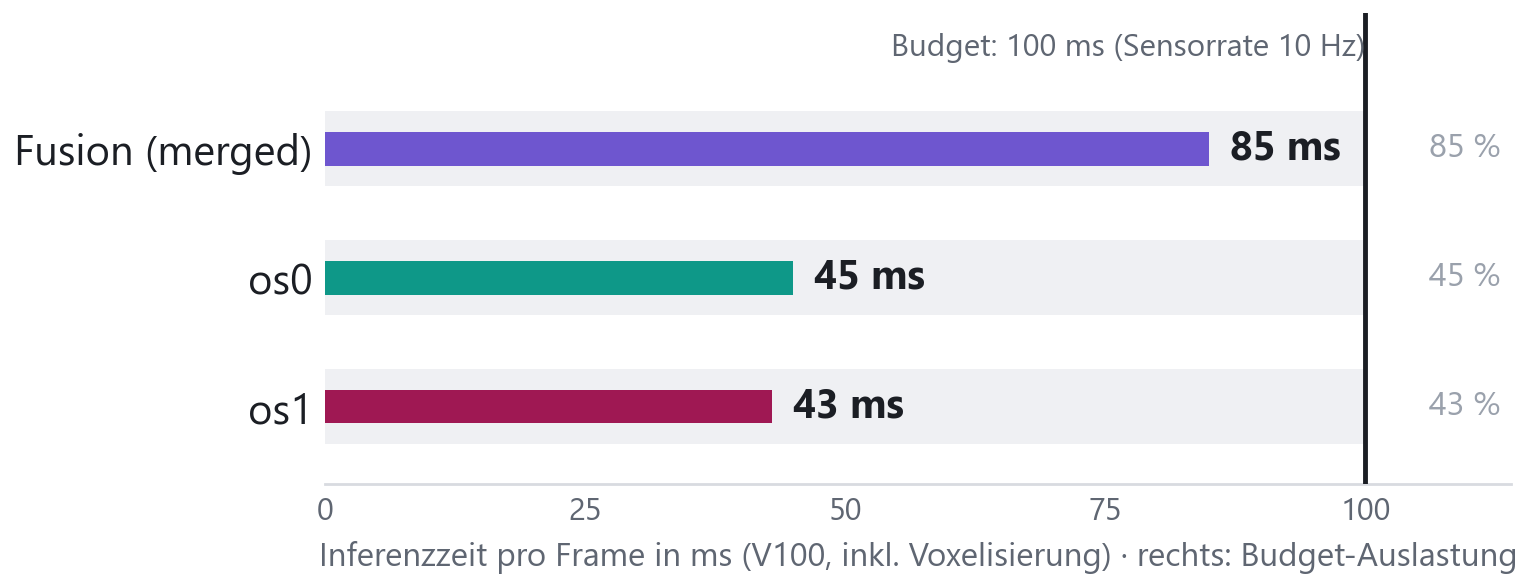
\includegraphics[width=0.95\textwidth]{images/inferenzzeit-budget.png}
\caption[Inferenzzeit im Verhältnis zum 100-ms-Budget]{Inferenzzeit je Frame im Verhältnis zum 100-ms-Budget einer 10-Hz-Sensorrate.}
\label{fig:inferenzzeit-budget}
\end{figure}

\subsection{Merge-Zeit und Ende-zu-Ende-Einordnung}

Die vorhandene Offline-Merge-Pipeline wurde auf einer lokalen CPU mit acht parallelen Workern gemessen. Die Messung umfasst 3.327 Frames, also alle verarbeiteten Rohframes und nicht nur die 2.122 Zeitstempel, die nach der Schnittmengenbildung über alle drei Ansichten für die Cross-Validation verbleiben. Über diese 3.327 Frames beträgt die mediane Bearbeitungszeit 2{,}25\,s pro Frame, der Mittelwert 2{,}20\,s, das Minimum 0{,}71\,s und das Maximum 4{,}00\,s. Enthalten sind PCD-Laden, statistischer Filter, feste Vorabtransformation, Downsampling, Normalenschätzung und per-Frame-ICP; die Registrierung dominiert die Zeit.

Es handelt sich um Einzelmessungen je Frame innerhalb eines Workers und nicht um eine aus der Gesamtlaufzeit abgeleitete Durchsatzkennzahl. Nur unter dieser Lesart lässt sich die Zahl im folgenden Absatz zu einer seriellen Latenz addieren. Dass der Median geringfügig über dem Mittelwert liegt, ist mit dieser Verteilung vereinbar: Die Zeiten sind nach unten hin gestreckt, das Minimum liegt 1{,}5\,s unter dem Median, das Maximum nur 1{,}75\,s darüber.

Der Wert ist stark hardwareabhängig. Die Vorgängerarbeit \cite{pagel2025railway} hat dieselbe Merge-Pipeline auf einer Server-CPU mit 72 Kernen gemessen und kam auf ungefähr 0{,}5\,s pro Frame. Die 2{,}25\,s sind damit keine inhärente Eigenschaft des Fusionsansatzes.

Würde diese Pipeline unverändert seriell vor der Inferenz ausgeführt, läge die Ende-zu-Ende-Latenz grob bei:

\begin{equation*}
    2{,}25\,\text{s Merge} + 0{,}085\,\text{s Inferenz} \approx 2{,}34\,\text{s pro Frame}
\end{equation*}

Das wäre nicht echtzeitfähig. Bei fest installierten Sensoren kann die Extrinsik jedoch einmalig offline bestimmt werden. Online wären dann nur Zeitsynchronisation, feste Transformation und Konkatenation erforderlich. Dieser optimierte Pfad wurde bislang nicht implementiert und gemessen.

Nach der \texttt{merged}-Inferenz verbleiben in einer seriellen 10-Hz-Pipeline nur ungefähr 15\,ms für Merge und sonstigen Overhead. Eine parallele CPU-/GPU-Pipeline könnte den Durchsatz verbessern, die Ende-zu-Ende-Latenz muss dennoch separat erfasst werden. Die korrekte Aussage ist deshalb:

\begin{quote}
    Die Modellinferenz auf bereits fusionierten Daten ist 10-Hz-fähig; die Echtzeitfähigkeit des vollständigen Online-Fusionssystems ist noch nicht nachgewiesen.
\end{quote}

\newpage
\section{Gültigkeit und Grenzen}
\label{sec:gueltigkeit}

\subsection{Interne Gültigkeit}

Für die Cross-Validation wurden folgende Schutzmaßnahmen umgesetzt:

\begin{itemize}
    \item vollständige Testexperimente sind von Training und Checkpoint-Auswahl ausgeschlossen,
    \item Train-, Validierungs- und Testframes sind disjunkt,
    \item GT-Sampling-Datenbanken enthalten ausschließlich Trainingsobjekte,
    \item ein zeitlicher Guard trennt Training und Validierung,
    \item der Zufallsseed ist fixiert,
    \item alle Ansichten verwenden dieselben gültigen physischen Zeitstempel,
    \item die offiziellen Fold-mAP-Werte wurden aus den Prediction-Dateien mit einer maximalen Abweichung von \(2{,}22 \times 10^{-16}\) reproduziert.
\end{itemize}

\subsection{Einschränkungen der Aussagekraft}

Die Ergebnisse besitzen folgende Grenzen:

\begin{enumerate}
    \item Alle neun Experimente stammen aus derselben Tiefgaragenszene. Die Cross-Validation misst Generalisierung auf ungesehene Aufnahmen und Trajektorien in dieser Szene, nicht auf neue Orte.
    \item Viele statische Fahrzeuge erscheinen in mehreren Folds an denselben Positionen. All-Object-Werte enthalten deshalb einen Anteil Szenenwiedererkennung.
    \item Die Zahl physisch verschiedener Zielobjekte und Personen ist klein.
    \item Person- und Fahrradlabels sind zwischen Ansichten nicht vollständig objektweise gepaart.
    \item Drei Folds erlauben nur eine vorsichtige Interpretation der Streuung und keine starke Signifikanzbehauptung.
    \item Je Fold und Ansicht wurde genau ein Trainingslauf mit dem festen Seed 42 durchgeführt. Die angegebene Standardabweichung erfasst deshalb ausschließlich die Streuung zwischen den Folds, nicht die zwischen verschiedenen Initialisierungen. Da der Fusionsvorsprung im Gesamt-mAP mit 0{,}021 kleiner ist als die Fold-Streuung von \texttt{merged} mit 0{,}037, wäre eine Wiederholung mit mehreren Seeds für eine belastbare Signifikanzaussage erforderlich.
    \item Gepoolte OOF-AP kombiniert Scores verschiedener Foldmodelle, die unterschiedlich kalibriert sein können. Die maßgeblichen Aussagen des Ergebniskapitels stützen sich deshalb auf Fold-Mittel; gepoolte Werte werden ergänzend berichtet.
    \item Experimentweise und gepoolte Auswertung beantworten verschiedene Fragen. Die experimentweise Auswertung berücksichtigt nur Frames, in denen die Zielklasse bewegt vorkommt, und übersieht Fehldetektionen außerhalb dieser Frames (Abschnitt~\ref{sec:os0-person}). Sie ist deshalb kein Ersatz für die Auswertung über die gesamte Testmenge.
    \item Die labelbasierte Bewegt-/Statisch-Variante wurde erst nach Sichtung des AP\textsubscript{60}-Artefakts definiert und wirkt zugunsten der fusionierten Ansicht. Sie ist deshalb kein vorab eingefrorener Bestandteil des Protokolls. Alle zentralen Aussagen werden daher zusätzlich unter der offiziellen Variante berichtet und bleiben dort bestehen.
    \item Der Vergleich zwischen finetunetem und ausschließlich vortrainiertem Modell in Abschnitt~\ref{sec:finetuning-wirkung} stützt sich auf Vergleichswerte aus \cite{pagel2025railway}. Diese wurden auf denselben Aufnahmen, aber nicht unter dem hier verwendeten Cross-Validation-Protokoll erhoben. Er ist deshalb als Größenordnungsvergleich zu lesen und nicht als kontrollierte Ablation.
    \item Die Live-Laufzeit des optimierten Online-Merges wurde noch nicht gemessen.
\end{enumerate}

\newpage
\section{Ausblick}

Die vorgelegte Arbeit zeigt, dass Multisensorfusion die beste ausgewogene Gesamtleistung für die 3D-Objekterkennung in einer stationären Tiefgaragenszene liefert. Auf dem Weg von dieser wissenschaftlichen Bewertung zu einem einsatzfähigen und besser generalisierenden System verbleiben mehrere Anschlussarbeiten, die im Folgenden umrissen werden.

\subsection{Finales Einsatzmodell}

Die Cross-Validation liefert mit dem Fold-Mittel von \(0{,}798 \pm 0{,}037\) für \texttt{merged} die wissenschaftliche Leistungsschätzung. Ein späterer produktiver Einsatz erfordert jedoch ein einzelnes finales Modell, das nicht auf zwei Dritteln der Daten trainiert wurde, sondern alle gültigen Aufnahmen nutzt. Der nächste logische Schritt ist daher ein Refit der gewählten Ansicht -- voraussichtlich \texttt{merged} -- auf sämtlichen validen Frames mit einer vorab festgelegten, der Cross-Validation entsprechenden Trainingsdauer.

Dieser finale Refit ist ausdrücklich nicht als neues unabhängiges Testergebnis zu verstehen. Die Cross-Validation bleibt die Leistungsschätzung; der Refit ist das spätere Inferenzartefakt. Die Trennung zwischen wissenschaftlicher Bewertung und produktivem Modelltraining ist eine bewährte Praxis und verhindert, dass das Testprotokoll nachträglich durch Kenntnis der Testergebnisse beeinflusst wird.

\subsection{Online-Merge und Echtzeitvalidierung}

Die aktuell gemessenen 85\,ms Inferenzzeit auf der fusionierten Punktwolke belegen die 10-Hz-Fähigkeit der Modellinferenz. Der vorgelagerte Merge-Schritt wurde jedoch bislang nur als Offline-Pipeline mit einer medianen Bearbeitungszeit von 2{,}25\,s pro Frame realisiert -- dominiert durch die per-Frame-ICP, die bei fest montierten Sensoren nicht erforderlich ist.

Für ein Live-System muss die Extrinsik einmalig auf einer geeigneten statischen Kalibrierszene bestimmt werden. Online verbleiben dann lediglich Zeitsynchronisation, feste Transformation und Konkatenation. Erst nach der Implementierung dieses optimierten Pfads kann eine belastbare Ende-zu-Ende-Latenzmessung durchgeführt werden. Bei einem 10-Hz-Sensortakt verbleiben nach der \texttt{merged}-Inferenz nur ungefähr 15\,ms für Merge und Overhead -- ob dieses Budget ausreicht, ist eine der zentralen offenen Fragen für den Produktivbetrieb.

\subsection{Tracking und zeitliche Filterung}

Die aktuelle Pipeline trifft Detektionsentscheidungen frameweise. Viele der in der Fehleranalyse dokumentierten Geisterboxen -- insbesondere kurzzeitig auftretende False Positives -- ließen sich durch zeitliche Konsistenz über mehrere Frames hinweg unterdrücken. Ein kalmanfilterbasiertes Tracking könnte Objekte über die Zeit verbinden, kurzlebige Einzelframe-Detektionen verwerfen und die verbleibenden Boxen räumlich glätten.

Darüber hinaus bietet das Tracking die Grundlage für Geschwindigkeitsschätzung und Trajektorienprädiktion -- beides relevante Größen für eine spätere verkehrstechnische Anwendung.

\subsection{Erweiterung der Datenbasis}

Die in Abschnitt~\ref{sec:gueltigkeit} genannte Beschränkung auf eine einzige Szene ist die gewichtigste Grenze dieser Arbeit. Die dokumentierte Ortsmemorierung in der Fehleranalyse zeigt, dass das Modell einen Teil seiner Leistung aus wiedererkannten Positionen zieht.

Ein belastbarer Generalisierungsnachweis erfordert die Aufnahme und Annotation weiterer Szenen -- im Idealfall an mehreren Standorten mit unterschiedlichen Raumabmessungen, Parkdichten und Untergründen. Nur so lässt sich bestimmen, ob das vortrainierte und finetunete Modell die zugrundeliegenden Formcharakteristiken der drei Zielklassen erfasst hat oder überwiegend szenenspezifische Muster memorierte. Die statischen Fahrzeuge, die in den aktuellen Daten an festen Positionen stehen, unterstreichen diese Notwendigkeit zusätzlich.

Die vorliegende Arbeit liefert mit der experiment-held-out Cross-Validation, der fusionierten Sicht und der dokumentierten Evaluationspipeline die methodische Grundlage, auf der diese Schritte aufbauen können.

\newpage
\section{Schlussfolgerung}

Das Projekt zeigt, dass ein auf KITTI vortrainiertes 3D-Detektionsmodell durch Finetuning erfolgreich auf eine fest installierte Tiefgaragenszene angepasst werden kann. Bezogen auf die vier eingangs gestellten Forschungsfragen ergibt sich folgendes Bild.

\paragraph{Wirkung des Finetunings.} Ausschließlich vortrainierte Modelle bleiben auf diesen Aufnahmen bei einem mAP von höchstens 0{,}058, das hier finetunete Modell erreicht 0{,}798 -- ein Abstand von 0{,}740 mAP. Der Abstand zwischen den beiden untersuchten Architekturen beträgt demgegenüber 0{,}047 bis 0{,}118 mAP und ist damit sechs- bis sechzehnmal kleiner. Die beiden Zahlen sind unterschiedlich abgesichert. Der Architekturvergleich ist kontrolliert: Beide Modelle unterscheiden sich ausschließlich in der Detektorarchitektur und stimmen in allen übrigen Festlegungen überein; seine Grenze ist die Verallgemeinerung, da nur zwei Vertreter derselben gitterbasierten Familie auf einer einzigen Szene geprüft wurden. Der Baselinewert dagegen stammt aus einer Vorgängerarbeit, die nicht unter diesem Protokoll und möglicherweise nicht mit derselben Datenkonvertierung und Metrik erhoben wurde; der kausale Beitrag des Finetunings ist damit nicht kontrolliert bestimmt. Bei einem Unterschied dieser Größe ist die Richtung dennoch eindeutig, und für vergleichbare stationäre Aufbauten legt das Ergebnis nahe, den Aufwand zunächst in Zieldaten und deren Annotation zu investieren, bevor Architekturen verglichen werden.

\paragraph{Einzelsensoren gegenüber Fusion.} PointPillars liefert mit der fusionierten Punktwolke in jedem Cross-Validation-Fold den höchsten Gesamt-mAP. Über alle Objekte beträgt der Vorsprung im Fold-Mittel 0{,}021. Beschränkt auf die bewegten Objekte und auf derselben Aggregationsstufe berechnet, wächst er auf 0{,}040 in der offiziellen und 0{,}069 in der labelbasierten Auswertung. Im Gesamtwert fällt der Unterschied zwischen den Ansichten damit kleiner aus. Dieser Wert bewertet zugleich die Wiedererkennung zahlreicher wiederkehrender geparkter Fahrzeuge; wie stark diese den Abstand beeinflussen, lässt sich wegen der nichtlinearen AP-Berechnung nicht isoliert bestimmen.

\paragraph{Finden gegenüber Lokalisieren.} Der Fusionsvorteil liegt in der räumlichen Präzision, nicht im Auffinden. Bei AP\textsubscript{30} erreichen alle Ansichten mindestens 0{,}65 und überwiegend mehr als 0{,}80; jede bewegte Klasse wird grundsätzlich aus jeder Perspektive gefunden. Auf den einzelnen Testexperimenten ist bei AP\textsubscript{30} sogar \texttt{os0} die stärkste und gleichmäßigste Ansicht (Mittel 0{,}914 bei einer Standardabweichung von 0{,}023 gegenüber 0{,}871 bei 0{,}063 für \texttt{merged}). Erst bei AP\textsubscript{60} führt \texttt{merged}, bei Person und Fahrrad mit erheblichem Abstand und in beiden Auswertungsvarianten. Beim Fahrrad sind die Varianten sogar identisch, weil keine statischen Fahrräder annotiert sind. Nur beim Auto kehrt die offizielle Variante die Rangfolge um, was auf ein aufgeklärtes Zuordnungsartefakt an einem geparkten Fahrzeug zurückgeht.

\paragraph{Fehlerbilder und Laufzeitgrenzen.} Die dominierenden Fehler sind Geisterboxen an Positionen, an denen in den Trainingsaufnahmen Objekte vorkamen, sowie klassenübergreifende Mehrfachhypothesen an dünn abgetasteten Fahrzeugkanten. Beide verweisen auf die Ein-Szenen-Datenbasis als Hauptbegrenzung. Die Modellinferenz ist mit 85\,ms auf der fusionierten Punktwolke 10-Hz-fähig; die Echtzeitfähigkeit des vollständigen Online-Fusionssystems ist dagegen nicht nachgewiesen, da der vorgelagerte Merge bislang nur als Offline-Pipeline mit 2{,}25\,s pro Frame existiert.

\bigskip

Die Fusion ist nicht erforderlich, um das bewegte Auto zu erkennen. In der experimentweisen Auswertung ist \texttt{os0} auf allen drei Autoaufnahmen sogar die stärkste Ansicht (AP\textsubscript{30} zwischen 0{,}92 und 0{,}96); in der gepoolten Auswertung über alle Testvorhersagen liegen die drei Ansichten mit 0{,}891, 0{,}885 und 0{,}832 dicht beieinander. Der frühere starke \texttt{os1}-Einbruch war ein Artefakt der zeitlich und räumlich gekoppelten Testaufteilung. Dieses Ergebnis unterstreicht, wie stark wissenschaftliche Schlussfolgerungen von einem passenden Evaluationsdesign abhängen.

Die aussagekräftigste Gesamtformulierung lautet:

\begin{quote}
    Die Multisensorfusion liefert die beste ausgewogene Gesamtleistung und erreicht bei Personen und Fahrrädern in beiden Auswertungsvarianten die präziseste Lokalisierung, ist aber nicht in jeder Klasse und bei jeder Metrik die beste Ansicht.
\end{quote}

Für einen späteren Einsatz sind vor allem ein finaler Refit des ausgewählten Modells, ein gemessener Online-Merge, validierungsbasierte Betriebsschwellen und zeitliches Tracking erforderlich.

\newpage
\section{Reproduzierbarkeit und Projektartefakte}

\subsection{Zentrale Implementierungen}

\begin{itemize}
    \item \textbf{Cross-Validation-Splits:}\\ \texttt{mmdetection3d/tools/dataset\_converters/}\\\texttt{create\_exp\_crossval\_splits.py}
    \item \textbf{PointPillars-CV-Konfiguration:}\\ \texttt{mmdetection3d/configs/pointpillars/}\\\texttt{pointpillars\_hv\_secfpn\_8xb6-50e\_exp-crossval-gtsample.py}
    \item \textbf{Trainingssteuerung:}\\ \texttt{mmdetection3d/tools/run\_exp\_crossval.sh}
    \item \textbf{Cross-Validation-Auswertung:}\\ \texttt{mmdetection3d/tools/analysis\_tools/exp\_eval\_crossval.py}
    \item \textbf{Geisterboxanalyse:}\\ \texttt{mmdetection3d/tools/analysis\_tools/exp\_ghost\_boxes\_crossval.py}
    \item \textbf{Punktwolken-Merge:} \texttt{experiment/pcd\_merge.py}
    \item \textbf{Label-Editor:} \texttt{experiment/manual\_bbox\_editor.py}
\end{itemize}

\subsection{Primäre Ergebnisquellen}

\begin{itemize}\raggedright
    \item \texttt{results/CROSS\_VALIDATION.md}: eingefrorenes Evaluationsprotokoll
    \item \texttt{results/CROSS\_VALIDATION\_RESULTS.md}: offizielle PointPillars-Ergebnisse
    \item \texttt{results/CROSS\_VALIDATION\_STATIC\_AWARE.md}: labelbasierte Teilbewertung
    \item \texttt{results/CENTERPOINT\_CV\_STATIC\_AWARE.md}: CenterPoint-Vergleich
    \item \texttt{results/GHOST\_BOXES.json}: generalisierte OOF-Fehlerzählung
    \item \texttt{results/DATA\_AUDIT.md}: Daten-, Metrik- und Ursachenanalyse
    \item \texttt{results/ABLATION\_BICYCLE.md}: frühere kontrollierte Ablationen
\end{itemize}

\subsection{Präsentationsmaterial}

Das primäre qualitative Video ist \texttt{results/videos/}\\\texttt{exp1\_cv\_full\_three\_views\_oblique.mp4}. Es zeigt alle 105 gemeinsamen gültigen Frames von Experiment 1 mit den drei Fold-1-Modellen, für die das vollständige Experiment während Training und Checkpoint-Auswahl ungesehen war. Abbildung~\ref{fig:drei-sichten} zeigt ein Standbild daraus.

\begin{figure}[H]
\centering
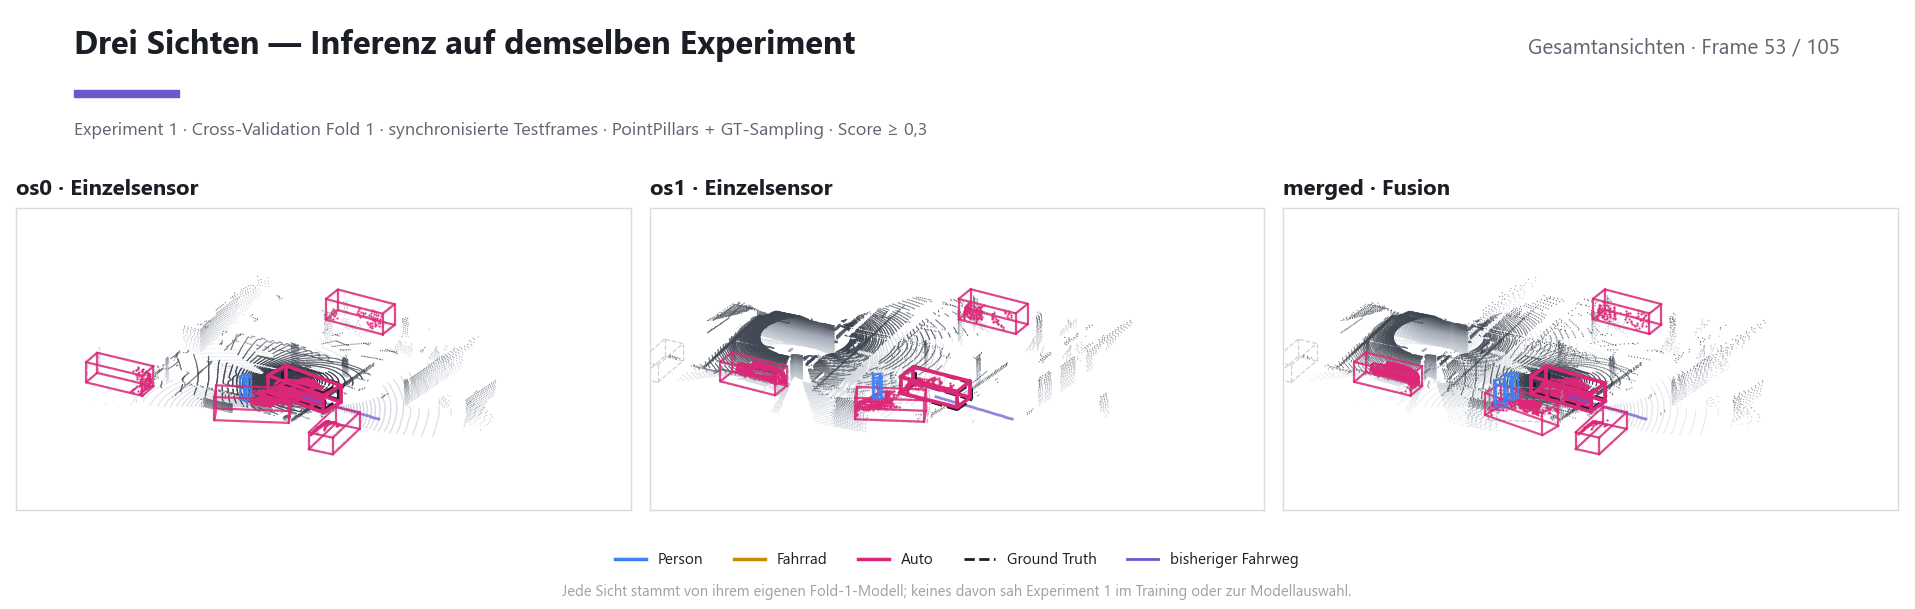
\includegraphics[width=\textwidth]{images/drei-sichten-standbild.png}
\caption{Standbild aus dem qualitativen Video: dieselbe Szene aus \texttt{os0}, \texttt{os1} und \texttt{merged}, jeweils vorhergesagt vom zugehörigen Fold-1-Modell.}
\label{fig:drei-sichten}
\end{figure}

Ältere Videos des temporalen 11-Frame-Testsegments sind nur historische Artefakte. Sie dürfen nicht als Beleg dafür verwendet werden, dass \texttt{os1} das bewegte Auto generell nicht erkennen könne.


\clearpage
\section*{Literaturverzeichnis}
\addcontentsline{toc}{section}{Literaturverzeichnis}
\printbibliography[heading=none]

\end{document}
